Celem tego rozdziału jest zaprezentowanie otrzymanych wyników wykrywania fiksacji, oraz dodatkowych danych statystycznych z nimi powiązanych, takich jak czas trwania algorytmu, wykorzystanie pamięci operacyjnej. Dodatkowo dla algorytmu uczenia maszynowego obliczona została jego precyzja. Do każdych z rezultatów została dołączona krótka analiza. Rozdział rozpoczęto od prezentacji stanowiska, na którym zostały przeprowadzone pomiary, a następnie stworzono krótką charakterystykę danych wejściowych. Kolejną część przeznaczono na opis wpływu parametrów wejściowych na otrzymane wyniki. Dalej stworzono krótką analizę wpływu źródła danych na łączny czas trwania algorytmu. W ostatniej sekcji porównano otrzymane wyniki oraz przeprowadzono ich analizę.\par
\section{Opis komputera}
Stworzenie oraz testy aplikacji wykrywającej fiksacje zostały przeprowadzone na maszynie zaprezentowanej w tabeli \ref{tab:machine}. Wymieniono w niej tylko elementy mogące wpłynąć na ostateczne wyniki, tzn. procesor wraz z jego taktowaniem, pamięć RAM, typ dysku twardego, na którym dane były przechowywane, jego prędkość obrotową. Pominięto takie elementy jak ilość rdzeni lub wątków, ze względu na jednowątkowość utworzonego projektu. Obecnie taką maszynę uznaje się za średnio-wydajną maszynę. Również pominięto prędkość odczytu z dysku SSD, pomimo znalezienia się na nim bazy danych, gdyż połącznenie jest wykonywane za pomocą protokołu \emph{http}.\par
\begin{table}[H]
    \centering
    \begin{tabular}{|l|l|}
        \hline
        Procesor       & Intel Core-i5 8600 @ 3.10 GHz          \\ \hline
        Pamięć RAM     & 16GB DDR4 @ 3200 MHz \\ \hline
        Typ dysku twardego           & HDD              \\ \hline
        Dysk twardy         & Toshiba HDWD110              \\ \hline
        Prędkość obrotowa         & 7200 obr./min              \\ \hline
    \end{tabular}
    \caption{Spis części komputera pomiarowego}
    \label{tab:machine}
\end{table}
\section{Parametry danych wejściowych}
\label{sec:entryparameters}
Dla każdego pliku umieszczonego w folderze \emph{\/data} w katalogu głównym aplikacji można określić następującą charakterystykę. Wykonane zostało 30 pomiarów punktów, w folderze istnieje 48 plików z pomiarami. Średnią ilością otrzymanych pomiarów, włącznie z punktami 'SS' jest 99059 pomiarów. Pomiary zostały wykonywane z częstotliwością 1000 Hz, czyli co 1 ms. W tabeli \ref{tab:measurementstats} zaprezentowano indywidualną liczbę pomiarów w każdym pliku.\par
{\footnotesize
\begin{longtable}{|l|r|}
    \hline
    \multicolumn{1}{|c|}{\textbf{Plik}} & \multicolumn{1}{c|}{\textbf{Liczba pomiarów}} \\ \hline
    \endfirsthead
    %
    \multicolumn{2}{c}%
    {{\bfseries Kontynuacja \thetable\ }} \\
    \hline
    \multicolumn{1}{|c|}{\textbf{Plik}} & \multicolumn{1}{c|}{\textbf{Liczba pomiarów}} \\ \hline
    \endhead
    %
    1\_01\_1311201811.cal & 99129 \\ \hline
    1\_02\_1310301856.cal & 99172 \\ \hline
    1\_03\_1310301904.cal & 99207 \\ \hline
    1\_04\_1310301810.cal & 99150 \\ \hline
    1\_05\_1310301817.cal & 99210 \\ \hline
    1\_06\_1310301837.cal & 99182 \\ \hline
    1\_12\_1310301901.cal & 99026 \\ \hline
    1\_14\_1310301912.cal & 99176 \\ \hline
    1\_15\_1310301840.cal & 99110 \\ \hline
    1\_16\_1310301844.cal & 99190 \\ \hline
    1\_17\_1310301825.cal & 99209 \\ \hline
    1\_20\_1310301822.cal & 99079 \\ \hline
    1\_21\_1310301833.cal & 99114 \\ \hline
    1\_22\_1310301908.cal & 99116 \\ \hline
    1\_23\_1310301722.cal & 98776 \\ \hline
    1\_24\_1311201804.cal & 99045 \\ \hline
    1\_25\_1311201806.cal & 99291 \\ \hline
    1\_26\_1311201835.cal & 98716 \\ \hline
    1\_27\_1311201823.cal & 99106 \\ \hline
    1\_28\_1310301813.cal & 98983 \\ \hline
    1\_29\_1310301914.cal & 99291 \\ \hline
    1\_31\_1310301807.cal & 99013 \\ \hline
    1\_32\_1310301831.cal & 99104 \\ \hline
    1\_34\_1310301804.cal & 99041 \\ \hline
    3\_01\_1401151823.cal & 99262 \\ \hline
    3\_02\_1401151905.cal & 98957 \\ \hline
    3\_03\_1401151858.cal & 99216 \\ \hline
    3\_04\_1401151803.cal & 98979 \\ \hline
    3\_05\_1401151752.cal & 99048 \\ \hline
    3\_06\_1311201818.cal & 98867 \\ \hline
    3\_12\_1401151843.cal & 98988 \\ \hline
    3\_14\_1401151837.cal & 99119 \\ \hline
    3\_15\_1401151641.cal & 98743 \\ \hline
    3\_16\_1401151847.cal & 98990 \\ \hline
    3\_17\_1401151814.cal & 99299 \\ \hline
    3\_20\_1401151759.cal & 98881 \\ \hline
    3\_21\_1401151911.cal & 99225 \\ \hline
    3\_22\_1401151828.cal & 99040 \\ \hline
    3\_23\_1401151854.cal & 99023 \\ \hline
    3\_24\_1401151840.cal & 98707 \\ \hline
    3\_25\_1401151908.cal & 99054 \\ \hline
    3\_26\_1401151826.cal & 99206 \\ \hline
    3\_27\_1401151811.cal & 99046 \\ \hline
    3\_28\_1401151747.cal & 98689 \\ \hline
    3\_29\_1401151833.cal & 98729 \\ \hline
    3\_31\_1401151755.cal & 98963 \\ \hline
    3\_32\_1401151808.cal & 99244 \\ \hline
    3\_34\_1401151805.cal & 99143 \\ \hline
    \caption{Statystyki pomiarów}
    \label{tab:measurementstats}\\
\end{longtable}
}
\section{Przeprowadzone pomiary}
W tym podrozdziale zostały zaprezentowane otrzymane wyniki, których format zaprezentowano w sekcji \ref{ssec:exitdata}. Dodatkowo do każdego wyniku została przygotowana krótka analiza wraz z zaprezentowaniem dopełniających parametrów wyników, umożliwiających lepszą interpretację rezultatów. Pierwszym elementem jest ukazanie wpływu parametrów wewnętrznych algorytmów na wyniki końcowe. Druga sekcja porównuje czasy trwania algorytmów, wraz z analizą przyczyn różnic w zmierzonych czasach. Następna sekcja opisuje wyniki obciążenia pamięciowego przez zaimplementowane algorytmy wykrywania fiksacji. W przedostatnim podrozdziale zanalizowano metody wprowadzania danych wejściowych do aplikacji. Ostatnia analiza dotyczy dokładności algorytmu uczenia maszynowego. Sekcję \ref{ssec:algorithms} przeznaczono na porównanie wyników otrzymanych w trzech algorytmach.
\subsection{Analiza wpływu parametrów algorytmów}
\label{ssec:queryparameters}
W poniższej sekcji zostanie zaprezentowany wpływ parametrów wewnętrznych algorytmów opisanych w sekcji \ref{ssec:algorithms}. Zbadany zostanie ten wpływ pod kątem różnic w obciązeniu pamięciowym przez algorytmy, porównania ilości elementów wyjściowych oraz czasu trwania algorytmów. Ten podrozdział został podzielony na 3 części, każda prezentująca algorytmy opisane w sekcji \ref{ssec:algorithms}. Uczenie maszynowe posiada czwartą część, precyzję wyników algorytmu. W celu prezentacji rezultatów wykorzystano pierwszych dziesięć plików opisanych w sekcji \ref{sec:entryparameters}.
\subsubsection{Algorytm I-VT}
\label{sssec:ivtresults}
Zgodnie z definicją algorytmu I-VT zaprezentowaną w sekcji \ref{ssec:ivt}, możemy zdefiniować jeden parametr wewnętrzny, który może wpływać na wyniki końcowe algorytmów. Tym parametrem jest próg prędkości międzypunktowej. W tym podrozdziale został zaprezentowany wpływ tego parametru na wyniki, a także przeprowadzono analizę wyników. Analizę wykonano dla wartości: \emph{v = 0.0001, 0.005, 0.001, 0.01}. \par
\textbf{Liczba wykrytych fiksacji}\par
W tabeli \ref{tab:ivtfixationcomparison} zaprezentowano wynik pomiaru liczby wykrytych fiksacji przeprowadzonej na dziesięciu plikach dla algorytmu I-VT. W pierwszej kolumnie umieszczono nazwę pliku, a w następnych zmierzoną liczbę fiksacji oraz sakad, względem odpowiedniej wartości parametru prędkości.
Jak można zauważyć dla tego algorytmu im mniejsza prędkość graniczna, tym więcej fiksacji jest wykrywanych. Jest to spowodowane tym iż, im mniejszy parametr tym mniejsza dokładność filtrowania punktów. Przykład takiej niskiej precyzji w oddzielaniu fiksacji od sakad zaprezentowano na rysunku \ref{fig:ivterrorresults}. Niedokładność tego wyniku polega na wykrywaniu jako fiksacji ruchu międzypunktowego. Ze względu na tylko jedno porównanie, zaprezentowane w warunku 3 pseudokodu \ref{lst:ivtpseudocode} należy określić dokładną wartość tej prędkości. Można dzięki temu stwierdzić, iż otrzymane wyniki są zgodne z oczekiwaniami.\par
\begin{figure}[H]
    \centering
    \captionsetup{justification=centering,margin=2cm}
    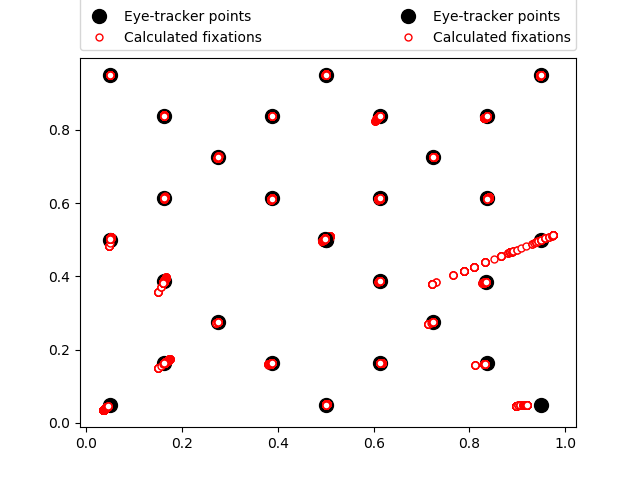
\includegraphics[width=\linewidth]{resources/ivt-errorresults.png}
    \caption{Błędne przedstawienie punktów dla algorytmu I-VT}
    \label{fig:ivterrorresults}
\end{figure}
Po zaobserwowaniu wyników graficznych w plikach wynikowych stwierdzono, iż parametr prędkości powinien znajdować się w okolicach wartości $v \in (0.005)$, gdyż dla tego wyniku zaobserwowano najdokładniejsze wyniki. Ostatnią badaną wartością było $v = 0.1$, jednak rezultatem takiego parametru było 0 lub 1 wykrytych fiksacji, dlatego zdecydowano się na pominięcie tej kolumny w tabeli \ref{tab:ivtfixationcomparison}.\par
{\small
\begin{longtable}{l|l|l|l|l|l|l|l|l|} 
    \cline{2-9}
     & \multicolumn{8}{c|}{\textbf{Ilość fiksacji/sakad}} \\ \hline
    \endfirsthead
    %
    \multicolumn{9}{c}%
    {{\bfseries Kontynuacja tabeli \thetable\ }} \\
    \cline{2-9}
     & \multicolumn{8}{c|}{\textbf{Ilość fiksacji/sakad}} \\ \hline
    \endhead
    %
    \multicolumn{1}{|c|}{\textbf{Plik}} & \multicolumn{2}{c|}{\textbf{v = 0,0001}} & \multicolumn{2}{c|}{\textbf{v = 0,005}} & \multicolumn{2}{c|}{\textbf{v = 0,001}} & \multicolumn{2}{l|}{\textbf{v = 0,01}} \\ \hline
    \multicolumn{1}{|l|}{1\_01\_1311201811.cal} & 6434 & \cellcolor[HTML]{EFEFEF}91444 & 780 & \cellcolor[HTML]{EFEFEF}3744 & 18015 & \cellcolor[HTML]{EFEFEF}52054 & 513 & \cellcolor[HTML]{EFEFEF}1545 \\ \hline
    \multicolumn{1}{|l|}{1\_02\_1310301856.cal} & 5896 & \cellcolor[HTML]{EFEFEF}92107 & 110 & \cellcolor[HTML]{EFEFEF}2415 & 1011 & \cellcolor[HTML]{EFEFEF}8817 & 37 & \cellcolor[HTML]{EFEFEF}405 \\ \hline
    \multicolumn{1}{|l|}{1\_03\_1310301904.cal} & 5645 & \cellcolor[HTML]{EFEFEF}92313 & 99 & \cellcolor[HTML]{EFEFEF}2027 & 1592 & \cellcolor[HTML]{EFEFEF}7547 & 54 & \cellcolor[HTML]{EFEFEF}446 \\ \hline
    \multicolumn{1}{|l|}{1\_04\_1310301810.cal} & 6792 & \cellcolor[HTML]{EFEFEF}90736 & 101 & \cellcolor[HTML]{EFEFEF}1688 & 1526 & \cellcolor[HTML]{EFEFEF}9217 & 30 & \cellcolor[HTML]{EFEFEF}263 \\ \hline
    \multicolumn{1}{|l|}{1\_05\_1310301817.cal} & 6475 & \cellcolor[HTML]{EFEFEF}91476 & 204 & \cellcolor[HTML]{EFEFEF}2877 & 11015 & \cellcolor[HTML]{EFEFEF}25880 & 85 & \cellcolor[HTML]{EFEFEF}939 \\ \hline
    \multicolumn{1}{|l|}{1\_06\_1310301837.cal} & 6815 & \cellcolor[HTML]{EFEFEF}90960 & 98 & \cellcolor[HTML]{EFEFEF}1889 & 3308 & \cellcolor[HTML]{EFEFEF}8590 & 42 & \cellcolor[HTML]{EFEFEF}288 \\ \hline
    \multicolumn{1}{|l|}{1\_12\_1310301901.cal} & 6726 & \cellcolor[HTML]{EFEFEF}91100 & 118 & \cellcolor[HTML]{EFEFEF}1865 & 6954 & \cellcolor[HTML]{EFEFEF}14511 & 42 & \cellcolor[HTML]{EFEFEF}399 \\ \hline
    \multicolumn{1}{|l|}{1\_14\_1310301912.cal} & 11964 & \cellcolor[HTML]{EFEFEF}82189 & 83 & \cellcolor[HTML]{EFEFEF}2213 & 278 & \cellcolor[HTML]{EFEFEF}6612 & 46 & \cellcolor[HTML]{EFEFEF}641 \\ \hline
    \multicolumn{1}{|l|}{1\_15\_1310301840.cal} & 7737 & \cellcolor[HTML]{EFEFEF}89751 & 87 & \cellcolor[HTML]{EFEFEF}1208 & 12041 & \cellcolor[HTML]{EFEFEF}22008 & 42 & \cellcolor[HTML]{EFEFEF}263 \\ \hline
    \multicolumn{1}{|l|}{1\_16\_1310301844.cal} & 6509 & \cellcolor[HTML]{EFEFEF}91431 & 126 & \cellcolor[HTML]{EFEFEF}1745 & 17453 & \cellcolor[HTML]{EFEFEF}42023 & 48 & \cellcolor[HTML]{EFEFEF}529 \\ \hline
    \caption{Wpływ parametru prędkości granicznej dla algorytmu I-VT, ilość fiksacji}
    \label{tab:ivtfixationcomparison}\\
\end{longtable}
}
\textbf{Analiza czasu trwania algorytmu}\par
W tabeli \ref{tab:ivttimecomparison} zaprezentowano wyniki pomiaru czasu trwania algorytmu I-VT dla różnych wartości prędkości progowej. Czas trwania zaprezentowano w sekundach. Obserwując otrzymane wyniki możemy stwierdzić, iż czas trwania algorytmu wzrasta odwrotnie proporcjonalnie do ilości wykrytych fiksacji. Zastanawiającym wynikiem jest pomiar czasu dla parametru $v = 0.01$, ze względu na podobieństwo do pomiarów z pierwszej kolumny. Prawdopodobnie jest to spowodowane niską liczbą elementów koniecznych do wykonania grupowania punktów, ze względu na stosunkowo duży parametr prędkości.\par
{\small
\begin{longtable}{l|l|l|l|l|}
    \cline{2-5}
     & \multicolumn{4}{c|}{\textbf{Pomiar długości trwania algorytmu (w s)}} \\ \hline
    \endfirsthead
    %
    \multicolumn{5}{c}%
    {{\bfseries Kontynuacja tabeli \thetable\ }} \\
    \cline{2-5}
     & \multicolumn{4}{c|}{\textbf{Pomiar długości trwania algorytmu (w s)}} \\ \hline
    \endhead
    %
    \multicolumn{1}{|c|}{\textbf{Plik}} & \multicolumn{1}{c|}{\textbf{v = 0,0001}} & \multicolumn{1}{c|}{\textbf{v = 0,005}} & \multicolumn{1}{c|}{\textbf{v = 0,001}} & \textbf{v = 0,01} \\ \hline
    \multicolumn{1}{|l|}{1\_01\_1311201811.cal} & 1.265625 & 4.21875 & 24.234375 & 3.515625 \\ \hline
    \multicolumn{1}{|l|}{1\_02\_1310301856.cal} & 1.203125 & 1.671875 & 4.375 & 1.5625 \\ \hline
    \multicolumn{1}{|l|}{1\_03\_1310301904.cal} & 1.15625 & 1.5625 & 6.203125 & 1.46875 \\ \hline
    \multicolumn{1}{|l|}{1\_04\_1310301810.cal} & 1.578125 & 1.546875 & 6.0625 & 1.5 \\ \hline
    \multicolumn{1}{|l|}{1\_05\_1310301817.cal} & 1.203125 & 1.921875 & 31.765625 & 1.625 \\ \hline
    \multicolumn{1}{|l|}{1\_06\_1310301837.cal} & 1.25 & 1.53125 & 12.3125 & 1.4375 \\ \hline
    \multicolumn{1}{|l|}{1\_12\_1310301901.cal} & 1.359375 & 1.546875 & 24.875 & 1.4375 \\ \hline
    \multicolumn{1}{|l|}{1\_14\_1310301912.cal} & 4.203125 & 1.484375 & 1.90625 & 1.5 \\ \hline
    \multicolumn{1}{|l|}{1\_15\_1310301840.cal} & 1.421875 & 1.421875 & 33.875 & 1.421875 \\ \hline
    \multicolumn{1}{|l|}{1\_16\_1310301844.cal} & 1.140625 & 1.46875 & 34.5625 & 1.453125 \\ \hline
    \caption{Wpływ parametru prędkości granicznej dla algorytmu I-VT, pomiar czasu}
    \label{tab:ivttimecomparison}\\
\end{longtable}
}
\textbf{Analiza wykorzystania pamięci operacyjnej}\par
Tabela \ref{tab:ivtmemorycomparison} przedstawia wyniki pomiaru wykorzystania pamięci przez algorytm I-VT. Jednostką pomiaru jest MiB. Zgodnie z zaobserwowanymi pomiarami, można stwierdzić, iż dla obecnych maszyn pomiar algorytmem I-VT nie stanowi zbytniego obciążenia, gdyż te pomiary wynoszą setki kilobajtów na cały pomiar, czyli około 90000 plików. Nie zauważono znaczącego wpływu parametru algorytmu na wykorzystanie pamięciowe, bo jak można zaobserwować, wartości w kolumnach nie posiadają specjalnej charakterystyki.\par
{\small
\begin{longtable}{l|l|l|l|l|}
    \cline{2-5}
     & \multicolumn{4}{c|}{\textbf{\begin{tabular}[c]{@{}c@{}}Wykorzystanie pamięci operacyjnej\\  (w MiB)\end{tabular}}} \\ \hline
    \endfirsthead
    %
    \multicolumn{5}{c}%
    {{\bfseries Kontynuacja tabeli \thetable\ }} \\
    \cline{2-5}
     & \multicolumn{4}{c|}{\textbf{\begin{tabular}[c]{@{}c@{}}Wykorzystanie pamięci operacyjnej\\  (w MiB)\end{tabular}}} \\ \hline
    \endhead
    %
    \multicolumn{1}{|c|}{\textbf{Plik}} & \multicolumn{1}{c|}{\textbf{v = 0,0001}} & \multicolumn{1}{c|}{\textbf{v = 0,005}} & \multicolumn{1}{c|}{\textbf{v = 0,001}} & \textbf{v = 0,01} \\ \hline
    \multicolumn{1}{|l|}{1\_01\_1311201811.cal} & 0.12500 & 0.17188 & 0.15234 & 0.21094 \\ \hline
    \multicolumn{1}{|l|}{1\_02\_1310301856.cal} & 0.10156 & 0.24609 & 0.16797 & 0.18359 \\ \hline
    \multicolumn{1}{|l|}{1\_03\_1310301904.cal} & 0.16016 & 0.15234 & 0.13281 & 0.12891 \\ \hline
    \multicolumn{1}{|l|}{1\_04\_1310301810.cal} & 0.19531 & 0.17188 & 0.12500 & 0.15625 \\ \hline
    \multicolumn{1}{|l|}{1\_05\_1310301817.cal} & 0.12109 & 0.15625 & 0.16406 & 0.24219 \\ \hline
    \multicolumn{1}{|l|}{1\_06\_1310301837.cal} & 0.06641 & 0.11328 & 0.12500 & 0.25000 \\ \hline
    \multicolumn{1}{|l|}{1\_12\_1310301901.cal} & 0.12500 & 0.22656 & 0.24219 & 0.17188 \\ \hline
    \multicolumn{1}{|l|}{1\_14\_1310301912.cal} & 0.20313 & 0.18750 & 0.21094 & 0.16016 \\ \hline
    \multicolumn{1}{|l|}{1\_15\_1310301840.cal} & 0.12109 & 0.12891 & 0.12891 & 0.21094 \\ \hline
    \multicolumn{1}{|l|}{1\_16\_1310301844.cal} & 0.10156 & 0.19922 & 0.17969 & 0.16797 \\ \hline
    \caption{Wpływ parametru prędkości granicznej dla algorytmu I-VT, wykorzystanie pamięci operacyjnej}
    \label{tab:ivtmemorycomparison}\\
\end{longtable}
}
\subsubsection{Algorytm I-DT}
\label{sssec:idtresults}
Algorytm I-DT różni się od algorytmu I-VT zaprezentowanego w sekcji \ref{sssec:ivtresults} tym, iż posiada on 2 parametry wewnętrzne: granicę dyspersji oraz czas trwania okna. W tej sekcji wyniki będą badane pod kątem modyfikacji tych dwóch parametrów. W tej sekcji badany będzie wpływ tych dwóch parametrów na otrzymane wyniki końcowe. W pierwszej części sprawdzany będzie wpływ parametru czasu trwania okna w odstępach co 50 ms, rozpoczynając od wartości 100 ms, kończąc na wartości 300 ms. Uznano, iż będzie ukazywać to dobrze różne wartości okna. Wartością dyspersji dla tego badania jest $D = 0.05$. W drugej części badany będzie wpływ wartości dyspersji na wyniki końcowe. Wartości dyspersji w tej części wynoszą odpowiednio \emph{0.01, 0.05, 0.1}. Punkty znajdujące się poniżej i powyżej tych wartości nie nadają się do dalszej analizy, gdyż dla mniejszych punktów otrzymujemy 0 fiksacji, a dla wartości \emph{1} osiągnięto po 3 fiksacje, przy czasie trwania 1000 sekund na plik. Dla tej części parametr rozmiaru okna wynosi 200 ms.\par

\textbf{Liczba wykrytych fiksacji - czas trwania okna}\par
W tabeli \ref{tab:idttimefixcomparison} zaprezentowano liczbę wykrytych fiksacji oraz sakad przez algorytm I-DT w zależności od parametru rozmiaru okna. Każda zależność od czasu okna została podzielona na dwie kolumny, odpowiednio fiksacje oraz sakady. Jak można zaobserwować w wynikach, wraz ze wzrostem rozmiaru okna, spada ilość wykrytych fiksacji. Wpływ na to ma umieszczenie punktów w oknie zgodnie z opisem zamieszczonym w rozdziale \ref{ssec:idt}. Im większe okno, tym więcej punktów w nim się znajduje, a skoro wyliczona fiksacja jest centroidem tego okna, to wynikiem tego algorytmu jest mniej fiksacji. Również liczba sakad jest zmniejszona od różnicy \emph{wszystkie punkty - fiksacje} ze względu na to, iż więcej punktów znajduje się w oknie i nie jest traktowanych jako sakady.\par
{\footnotesize
\begin{longtable}{|l|l|l|l|l|l|l|l|l|l|l|}
    \hline
     & \multicolumn{10}{c|}{\textbf{Liczba wykrytych fiksacji/sakad}} \\ \hline
    \endfirsthead
    %
    \multicolumn{11}{c}%
    {{\bfseries Kontynuacja tabeli \thetable\ }} \\
    \hline
     & \multicolumn{10}{c|}{\textbf{Liczba wykrytych fiksacji/sakad}} \\ \hline
    \endhead
    %
    \multicolumn{1}{|c|}{\textbf{Plik}} & \multicolumn{2}{c|}{\textbf{100}} & \multicolumn{2}{c|}{\textbf{150}} & \multicolumn{2}{c|}{\textbf{200}} & \multicolumn{2}{c|}{\textbf{250}} & \multicolumn{2}{c|}{\textbf{300}} \\ \hline
    1\_01\_1311201811.cal & 232 & \cellcolor[HTML]{EFEFEF}41639 & 151 & \cellcolor[HTML]{EFEFEF}51478 & 108 & \cellcolor[HTML]{EFEFEF}62301 & 84 & \cellcolor[HTML]{EFEFEF}70311 & 20 & \cellcolor[HTML]{EFEFEF}91783 \\ \hline
    1\_02\_1310301856.cal & 79 & \cellcolor[HTML]{EFEFEF}53260 & 46 & \cellcolor[HTML]{EFEFEF}56741 & 30 & \cellcolor[HTML]{EFEFEF}59877 & 28 & \cellcolor[HTML]{EFEFEF}63884 & 23 & \cellcolor[HTML]{EFEFEF}66419 \\ \hline
    1\_03\_1310301904.cal & 133 & \cellcolor[HTML]{EFEFEF}30814 & 98 & \cellcolor[HTML]{EFEFEF}38404 & 85 & \cellcolor[HTML]{EFEFEF}37146 & 73 & \cellcolor[HTML]{EFEFEF}44526 & 70 & \cellcolor[HTML]{EFEFEF}44934 \\ \hline
    1\_04\_1310301810.cal & 115 & \cellcolor[HTML]{EFEFEF}39130 & 85 & \cellcolor[HTML]{EFEFEF}38721 & 62 & \cellcolor[HTML]{EFEFEF}42761 & 56 & \cellcolor[HTML]{EFEFEF}48617 & 53 & \cellcolor[HTML]{EFEFEF}47580 \\ \hline
    1\_05\_1310301817.cal & 107 & \cellcolor[HTML]{EFEFEF}37975 & 81 & \cellcolor[HTML]{EFEFEF}44105 & 61 & \cellcolor[HTML]{EFEFEF}50329 & 52 & \cellcolor[HTML]{EFEFEF}51646 & 45 & \cellcolor[HTML]{EFEFEF}54772 \\ \hline
    1\_06\_1310301837.cal & 84 & \cellcolor[HTML]{EFEFEF}63589 & 58 & \cellcolor[HTML]{EFEFEF}65821 & 39 & \cellcolor[HTML]{EFEFEF}69476 & 33 & \cellcolor[HTML]{EFEFEF}70490 & 31 & \cellcolor[HTML]{EFEFEF}72190 \\ \hline
    1\_12\_1310301901.cal & 82 & \cellcolor[HTML]{EFEFEF}45263 & 61 & \cellcolor[HTML]{EFEFEF}46338 & 57 & \cellcolor[HTML]{EFEFEF}43221 & 47 & \cellcolor[HTML]{EFEFEF}48092 & 44 & \cellcolor[HTML]{EFEFEF}50457 \\ \hline
    1\_14\_1310301912.cal & 85 & \cellcolor[HTML]{EFEFEF}48028 & 58 & \cellcolor[HTML]{EFEFEF}54627 & 42 & \cellcolor[HTML]{EFEFEF}59476 & 31 & \cellcolor[HTML]{EFEFEF}65319 & 27 & \cellcolor[HTML]{EFEFEF}64586 \\ \hline
    1\_15\_1310301840.cal & 144 & \cellcolor[HTML]{EFEFEF}36881 & 116 & \cellcolor[HTML]{EFEFEF}42391 & 95 & \cellcolor[HTML]{EFEFEF}45018 & 83 & \cellcolor[HTML]{EFEFEF}50141 & 70 & \cellcolor[HTML]{EFEFEF}52791 \\ \hline
    1\_16\_1310301844.cal & 151 & \cellcolor[HTML]{EFEFEF}27608 & 122 & \cellcolor[HTML]{EFEFEF}32658 & 95 & \cellcolor[HTML]{EFEFEF}38068 & 80 & \cellcolor[HTML]{EFEFEF}40244 & 68 & \cellcolor[HTML]{EFEFEF}46049 \\ \hline
    \caption{Wpływ parametru czasu okna, algorytm I-DT, wyniki}
    \label{tab:idttimefixcomparison}\\
\end{longtable}
}\par
Na rysunku \ref{fig:idtt200} zaprezentowano przykładowy wynik tego algorytmu dla wartości $T = 200$.
\begin{figure}[H]
    \centering
    \captionsetup{justification=centering,margin=2cm}
    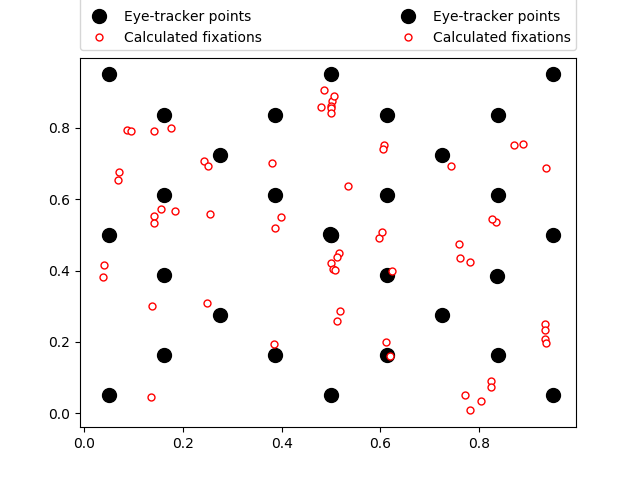
\includegraphics[width=0.8\linewidth]{resources/idt/idt-time-200-04.png}
    \caption{Wynik algorytmu I-DT, T = 200}
    \label{fig:idtt200}
\end{figure}
\begin{figure}[H]
    \centering
    \captionsetup{justification=centering,margin=2cm}
    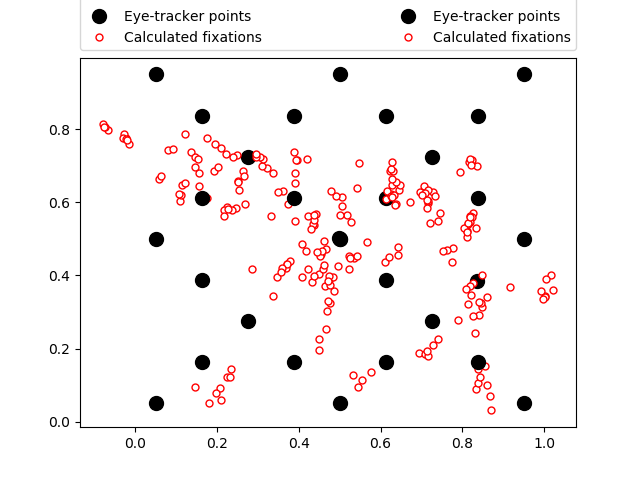
\includegraphics[width=0.8\linewidth]{resources/idt/idt-time-100-1_01-incorrect.png}
    \caption{Niepoprawny wynik algorytmu I-DT}
    \label{fig:idtweird}
\end{figure}
\textbf{Analiza czasów trwania algorytmu - czas trwania okna}\par
Tablica \ref{tab:idttimetimecomparison} zawiera zmierzony czas trwania algorytmu I-DT w zależności od rozmiaru okna. Podczas gdy pierwszy punkt wydaje się być anomalią, jak zaprezentowano na rysunku \ref{fig:idtweird}, nie znaleziono przyczyny tak niskich pomiarów czasu wykonywania.\par
Reszta zmierzonego czasu trwania algorytmu oscyluje w okolicach 200-300 sekund, co pozwala określić ten algorytm jako wolny, ale dokładny, ze względu na małą liczbę fiksacji zaprezentowaną w tabeli \ref{tab:idttimefixcomparison}.\par
{\footnotesize
\begin{longtable}{l|l|l|l|l|l|}
    \cline{2-6}
     & \multicolumn{5}{c|}{\textbf{Czas trwania algorytmu (w s)}} \\ \hline
    \endfirsthead
    %
    \multicolumn{6}{c}%
    {{\bfseries Kontynuacja tabeli \thetable\ }} \\
    \cline{2-6}
     & \multicolumn{5}{c|}{\textbf{Czas trwania algorytmu (w s)}} \\ \hline
    \endhead
    %
    \multicolumn{1}{|c|}{\textbf{Plik}} & \multicolumn{1}{c|}{\textbf{100}} & \multicolumn{1}{c|}{\textbf{150}} & \multicolumn{1}{c|}{\textbf{200}} & \multicolumn{1}{c|}{\textbf{250}} & \multicolumn{1}{c|}{\textbf{300}} \\ \hline
    \multicolumn{1}{|l|}{1\_01\_1311201811.cal} & 39.734375 & 35.734375 & 23.1875 & 13.265625 & 3.546875 \\ \hline
    \multicolumn{1}{|l|}{1\_02\_1310301856.cal} & 345.546875 & 354.015625 & 345.328125 & 365.359375 & 349.40625 \\ \hline
    \multicolumn{1}{|l|}{1\_03\_1310301904.cal} & 223.84375 & 216.15625 & 209.59375 & 220.234375 & 189.734375 \\ \hline
    \multicolumn{1}{|l|}{1\_04\_1310301810.cal} & 264.78125 & 243.984375 & 247.3125 & 247.765625 & 228.765625 \\ \hline
    \multicolumn{1}{|l|}{1\_05\_1310301817.cal} & 246.1875 & 254.265625 & 227.453125 & 240.96875 & 231.15625 \\ \hline
    \multicolumn{1}{|l|}{1\_06\_1310301837.cal} & 382.828125 & 371.15625 & 377.578125 & 372.875 & 350.765625 \\ \hline
    \multicolumn{1}{|l|}{1\_12\_1310301901.cal} & 313.765625 & 305.515625 & 291.9375 & 304.3125 & 299.34375 \\ \hline
    \multicolumn{1}{|l|}{1\_14\_1310301912.cal} & 386.15625 & 404.671875 & 404.0 & 407.734375 & 373.71875 \\ \hline
    \multicolumn{1}{|l|}{1\_15\_1310301840.cal} & 220.328125 & 221.0 & 215.703125 & 209.234375 & 195.1875 \\ \hline
    \multicolumn{1}{|l|}{1\_16\_1310301844.cal} & 193.15625 & 186.0625 & 182.734375 & 171.96875 & 166.328125 \\ \hline
    \caption{Wpływ parametru czasu okna, algorytm I-DT, czas trwania}
    \label{tab:idttimetimecomparison}\\
\end{longtable}
}
\textbf{Analiza obciążenia pamięci - czas trwania okna}\par
W tej sekcji zaprezentowano różnicę w obciążeniu pamięci operacyjnej dla algorytmu I-DT w zależności od parametru rozmiaru czasowego okna. Wynik tego pomiaru umieszczono w tabeli \ref{tab:idttimetimecomparison}. Przeglądając wyniki możemy zaobserwować brak zmian pomiędzy różnymi wynikami, co pozwala nam wywnioskować, iż nie ma żadnej korelacji między parametrem okna, a zużyciem pamięci.\par
{\small
\begin{longtable}{l|l|l|l|l|l|}
    \cline{2-6}
     & \multicolumn{5}{c|}{\textbf{\begin{tabular}[c]{@{}c@{}}Wykorzystanie pamięci operacyjnej\\  (w MiB)\end{tabular}}} \\ \hline
    \endfirsthead
    %
    \multicolumn{6}{c}%
    {{\bfseries Kontynuacja tabeli \thetable\ }} \\
    \cline{2-6}
     & \multicolumn{5}{c|}{\textbf{\begin{tabular}[c]{@{}c@{}}Wykorzystanie pamięci operacyjnej\\  (w MiB)\end{tabular}}} \\ \hline
    \endhead
    %
    \multicolumn{1}{|c|}{\textbf{Plik}} & \multicolumn{1}{c|}{\textbf{100}} & \multicolumn{1}{c|}{\textbf{150}} & \multicolumn{1}{c|}{\textbf{200}} & \multicolumn{1}{c|}{\textbf{250}} & \multicolumn{1}{c|}{\textbf{300}} \\ \hline
    \multicolumn{1}{|l|}{1\_01\_1311201811.cal} & 0.07031 & 0.07813 & 0.07422 & 0.07031 & 0.00781 \\ \hline
    \multicolumn{1}{|l|}{1\_02\_1310301856.cal} & 0.13281 & 0.07813 & 0.07422 & 0.08984 & 0.10938 \\ \hline
    \multicolumn{1}{|l|}{1\_03\_1310301904.cal} & 0.21484 & 0.13672 & 0.10938 & 0.13672 & 0.08984 \\ \hline
    \multicolumn{1}{|l|}{1\_04\_1310301810.cal} & 0.11719 & 0.13281 & 0.11719 & 0.10938 & 0.14063 \\ \hline
    \multicolumn{1}{|l|}{1\_05\_1310301817.cal} & 0.14063 & 0.12109 & 0.14063 & 0.24219 & 0.12891 \\ \hline
    \multicolumn{1}{|l|}{1\_06\_1310301837.cal} & 0.16016 & 0.07031 & 0.16406 & 0.08594 & 0.10547 \\ \hline
    \multicolumn{1}{|l|}{1\_12\_1310301901.cal} & 0.16797 & 0.16797 & 0.12891 & 0.16016 & 0.12891 \\ \hline
    \multicolumn{1}{|l|}{1\_14\_1310301912.cal} & 0.11719 & 0.12109 & 0.00000 & 0.12500 & 0.10156 \\ \hline
    \multicolumn{1}{|l|}{1\_15\_1310301840.cal} & 0.12109 & 0.08984 & 0.10156 & 0.09375 & 0.15625 \\ \hline
    \multicolumn{1}{|l|}{1\_16\_1310301844.cal} & 0.12891 & 0.09766 & 0.20703 & 0.11719 & 0.10156 \\ \hline
    \caption{Wpływ parametru czasu okna, algorytm I-DT, zużycie pamięci}
    \label{tab:idttimememorycomparison}\\
\end{longtable}
}
\textbf{Liczba wykrytych fiksacji - dyspersja}\par
W tabeli \ref{tab:idtdispfixcomparison} zaprezentowano wyniki algorytmu I-DT w zależności od wartości parametru dyspersji. Analogicznie do innych tabel dotyczących fiksacji i sakad przedstawionych w tym rozdziale wewnętrzne komórki zostały podzielone na wykryte fiksacje oraz sakady. Odczytując wyniki można wywnioskować, iż zmniejszanie parametru dyspersji powoduje zwiększenie ilości wykrytych fiksacji. Jest to spowodowane porównywaniem wartości dyspersji wewnątrz okna, więc logicznym następstwem tego rozwiązania jest, im mniejszy wymagany parametr dyspersji, tym więcej punktów można wykryć jako fiksacje. Wyniki dla pliku 1 i 10 zostaną przeanalizowane dla tabeli \ref{tab:idtdispmemorycomparison}.\par
{\small
\begin{longtable}{|l|l|l|l|l|l|l|}
    \hline
     & \multicolumn{6}{c|}{\textbf{Liczba wykrytych fiksacji/sakad}} \\ \hline
    \endfirsthead
    %
    \multicolumn{7}{c}%
    {{\bfseries Kontynuacja tabeli \thetable\ }} \\
    \hline
     & \multicolumn{6}{c|}{\textbf{Liczba wykrytych fiksacji/sakad}} \\ \hline
    \endhead
    %
    \multicolumn{1}{|c|}{\textbf{Plik}} & \multicolumn{2}{c|}{\textbf{D = 0.1}} & \multicolumn{2}{c|}{\textbf{D = 0.05}} & \multicolumn{2}{c|}{\textbf{D = 0.01}} \\ \hline
    1\_01\_1311201811.cal & 134 & \cellcolor[HTML]{EFEFEF}50061 & 108 & \cellcolor[HTML]{EFEFEF}62301 & 0 & \cellcolor[HTML]{EFEFEF}99129 \\ \hline
    1\_02\_1310301856.cal & 22 & \cellcolor[HTML]{EFEFEF}71070 & 30 & \cellcolor[HTML]{EFEFEF}59877 & 137 & \cellcolor[HTML]{EFEFEF}53162 \\ \hline
    1\_03\_1310301904.cal & 36 & \cellcolor[HTML]{EFEFEF}63871 & 85 & \cellcolor[HTML]{EFEFEF}37146 & 43 & \cellcolor[HTML]{EFEFEF}88033 \\ \hline
    1\_04\_1310301810.cal & 39 & \cellcolor[HTML]{EFEFEF}59185 & 62 & \cellcolor[HTML]{EFEFEF}42761 & 91 & \cellcolor[HTML]{EFEFEF}70730 \\ \hline
    1\_05\_1310301817.cal & 39 & \cellcolor[HTML]{EFEFEF}57755 & 61 & \cellcolor[HTML]{EFEFEF}50329 & 34 & \cellcolor[HTML]{EFEFEF}89663 \\ \hline
    1\_06\_1310301837.cal & 28 & \cellcolor[HTML]{EFEFEF}81731 & 39 & \cellcolor[HTML]{EFEFEF}69476 & 129 & \cellcolor[HTML]{EFEFEF}59483 \\ \hline
    1\_12\_1310301901.cal & 18 & \cellcolor[HTML]{EFEFEF}77708 & 57 & \cellcolor[HTML]{EFEFEF}43221 & 79 & \cellcolor[HTML]{EFEFEF}77443 \\ \hline
    1\_14\_1310301912.cal & 23 & \cellcolor[HTML]{EFEFEF}87308 & 42 & \cellcolor[HTML]{EFEFEF}59476 & 130 & \cellcolor[HTML]{EFEFEF}50360 \\ \hline
    1\_15\_1310301840.cal & 28 & \cellcolor[HTML]{EFEFEF}68066 & 95 & \cellcolor[HTML]{EFEFEF}45018 & 18 & \cellcolor[HTML]{EFEFEF}94418 \\ \hline
    1\_16\_1310301844.cal & 49 & \cellcolor[HTML]{EFEFEF}55464 & 95 & \cellcolor[HTML]{EFEFEF}38068 & 2 & \cellcolor[HTML]{EFEFEF}98779 \\ \hline
    \caption{Wpływ parametru dyspersji, algorytm I-DT, wyniki}
    \label{tab:idtdispfixcomparison}\\
\end{longtable}
}
\textbf{Analiza obciążenia pamięci - dyspersja}\par
Tabela \ref{tab:idtdispmemorycomparison} prezentuje otrzymane wyniki pomiaru wykorzystania pamięci przez algorytm I-DT, mając na uwadze różnice w parametrze dyspersji. Przeglądając wyniki, możemy zauważyć lekki spadek w otrzymanych wartościach pomiędzy drugą a trzecią kolumną. Pomimo zaobserwowanego zwiększenia liczby otrzymanych fiksacji wyświetlonego w tabeli \ref{tab:idtdispfixcomparison}, możemy zauważyć spadek w wykorzystaniu pamięciowym. Dzięki temu, można określić dla niektóych wartości, iż parametr dyspersji ma wpływ na zużycie pamięci operacyjnej. Wniosek dotyczący porównywania wartości dyspersji wewnątrz okna zaprezentowany przy okazji analizy tabeli \ref{tab:idtdispfixcomparison} można również zastosować do tabeli \ref{tab:idtdispmemorycomparison}.\par
{\small
\begin{longtable}{|l|l|l|l|}
    \hline
     & \multicolumn{3}{c|}{\textbf{\begin{tabular}[c]{@{}c@{}}Wykorzystanie pamięci obliczeniowej \\ (w MiB)\end{tabular}}} \\ \hline
    \endfirsthead
    %
    \multicolumn{4}{c}%
    {{\bfseries Kontynuacja tabeli \thetable\ }} \\
    \hline
     & \multicolumn{3}{c|}{\textbf{\begin{tabular}[c]{@{}c@{}}Wykorzystanie pamięci obliczeniowej \\ (w MiB)\end{tabular}}} \\ \hline
    \endhead
    %
    \multicolumn{1}{|c|}{\textbf{Plik}} & \multicolumn{1}{c|}{\textbf{D = 0.1}} & \multicolumn{1}{c|}{\textbf{D = 0.05}} & \multicolumn{1}{c|}{\textbf{D = 0.01}} \\ \hline
    1\_01\_1311201811.cal & 0,07031 & 0,07422 & 0,00000 \\ \hline
    1\_02\_1310301856.cal & 0,13281 & 0,07422 & 0,06641 \\ \hline
    1\_03\_1310301904.cal & 0,21484 & 0,10938 & 0,00391 \\ \hline
    1\_04\_1310301810.cal & 0,11719 & 0,11719 & 0,05078 \\ \hline
    1\_05\_1310301817.cal & 0,14063 & 0,14063 & 0,01563 \\ \hline
    1\_06\_1310301837.cal & 0,16016 & 0,16406 & 0,06641 \\ \hline
    1\_12\_1310301901.cal & 0,16797 & 0,12891 & 0,06641 \\ \hline
    1\_14\_1310301912.cal & 0,11719 & 0,00000 & 0,08984 \\ \hline
    1\_15\_1310301840.cal & 0,12109 & 0,10156 & 0,01563 \\ \hline
    1\_16\_1310301844.cal & 0,12891 & 0,20703 & 0,00000 \\ \hline
    \caption{Wpływ parametru dyspersji, algorytm I-DT, obciązenie pamięciowe}
    \label{tab:idtdispmemorycomparison}\\
\end{longtable}
}
\textbf{Analiza czasów trwania algorytmu - dyspersja}\par
Czasy trwania algorytmu I-DT dla różnych wartości dyspersji zaprezentowano w tabeli \ref{tab:idtdisptimecomparison}. Analizując otrzymane wartości, można wywnioskować, iż w parze z mniejszą wartością dyspersji idzie zmniejszenie czasu trwania algorytmu. Potwierdza to wstęp do tej analizy, gdzie dla wartości $D = 1$, zmierzono czas około 1000 sekund. Mniejsza ilość porównań jest powodem zależności dyspersji od czasu.\par
{\small
\begin{longtable}{|l|l|l|l|}
    \hline
     & \multicolumn{3}{c|}{\textbf{Czas trwania algorytmu (w s)}} \\ \hline
    \endfirsthead
    %
    \multicolumn{4}{c}%
    {{\bfseries Table \thetable\ continued from previous page}} \\
    \hline
     & \multicolumn{3}{c|}{\textbf{Czas trwania algorytmu (w s)}} \\ \hline
    \endhead
    %
    \multicolumn{1}{|c|}{\textbf{Plik}} & \multicolumn{1}{c|}{\textbf{D = 0.1}} & \multicolumn{1}{c|}{\textbf{D = 0.05}} & \multicolumn{1}{c|}{\textbf{D = 0.01}} \\ \hline
    1\_01\_1311201811.cal & 35.296875 & 23.1875 & 1.421875 \\ \hline
    1\_02\_1310301856.cal & 432.015625 & 345.328125 & 30.125 \\ \hline
    1\_03\_1310301904.cal & 501.46875 & 209.59375 & 4.53125 \\ \hline
    1\_04\_1310301810.cal & 397.765625 & 247.3125 & 17.125 \\ \hline
    1\_05\_1310301817.cal & 376.671875 & 227.453125 & 5.15625 \\ \hline
    1\_06\_1310301837.cal & 544.515625 & 377.578125 & 21.296875 \\ \hline
    1\_12\_1310301901.cal & 575.140625 & 291.9375 & 9.3125 \\ \hline
    1\_14\_1310301912.cal & 636.828125 & 404.0 & 43.46875 \\ \hline
    1\_15\_1310301840.cal & 491.1875 & 215.703125 & 3.4375 \\ \hline
    1\_16\_1310301844.cal & 356.453125 & 182.734375 & 1.34375 \\ \hline
    \caption{Wpływ parametru dyspersji, algorytm I-DT, czas trwania}
    \label{tab:idtdisptimecomparison}\\
\end{longtable}
}
\subsubsection{Algorytm ML - wpływ parametru prędkości}
\label{sssec:mlivt}
Ze względu na konieczność określenia klasy przynależności dla punktu, tzn. czy należy on do fiksacji, należało wyznaczyć fiksację dowolnym algorytmem. Ze względu na prostotę obliczeń oraz małą złożoność czasową, zdecydowano się na wstępną analizę algorytmem I-VT. Analizę bezpośredniego wpływu parametru wewnętrznego na algorytm I-VT zaprezentowano w sekcji \ref{sssec:ivtresults}. Wyniki są podane dla parametru podziału danych: 50\% danych testowych, 50\% danych treningowych.\par
\textbf{Liczba wykrytych fiksacji}\par
Jak zaprezentowano w tabeli \ref{tab:mlivtfixcomparison}, otrzymane wyniki pozwalają stwierdzić, iż parametr progowy prędkości międzypunktowej nie wpływa znacząco na wyniki końcowe algorytmu. Ciekawym efektem ubocznym zmiany parametru, zaobserwowanym w ostatnich kolumnach tabeli \ref{tab:mlivtfixcomparison} jest brak otrzymanych wyników końcowych ze względu na otrzymany wyjątek w trakcie tworzenia listy punktów końcowych. Także zaobserwowano znaczący przyrost liczby fiksacji względem sakad, prawdopodobnie jest to spowodowane zbyt małą próbką danych typu \emph{"punkt należy do fiksacji"}, co przedstawiono w ostatnich kolumnach tabeli \ref{tab:ivtfixationcomparison}.\par
{\small
\begin{longtable}{l|l|l|l|l|l|l|l|l|}
    \cline{2-9}
     & \multicolumn{8}{c|}{\textbf{Liczba wykrytych fiksacji/sakad}} \\ \hline
    \endfirsthead
    %
    \multicolumn{9}{c}%
    {{\bfseries Kontynuacja tabeli \thetable\ }} \\
    \cline{2-9}
     & \multicolumn{8}{c|}{\textbf{Liczba wykrytych fiksacji/sakad}} \\ \hline
    \endhead
    %
    \multicolumn{1}{|c|}{\textbf{Plik}} & \multicolumn{2}{c|}{\textbf{v = 0,00001}} & \multicolumn{2}{c|}{\textbf{v = 0,0005}} & \multicolumn{2}{c|}{\textbf{v = 0,0001}} & \multicolumn{2}{l|}{\textbf{v = 0,005}} \\ \hline
    \multicolumn{1}{|l|}{1\_01\_1311201811.cal} & 3809 & \cellcolor[HTML]{EFEFEF}95319 & 3800 & \cellcolor[HTML]{EFEFEF}95328 & 3801 & \cellcolor[HTML]{EFEFEF}95327 &  & \cellcolor[HTML]{EFEFEF} \\ \hline
    \multicolumn{1}{|l|}{1\_02\_1310301856.cal} & 3336 & \cellcolor[HTML]{EFEFEF}95835 & 3345 & \cellcolor[HTML]{EFEFEF}95826 & 3433 & \cellcolor[HTML]{EFEFEF}95738 & 97942 & \cellcolor[HTML]{EFEFEF}1229 \\ \hline
    \multicolumn{1}{|l|}{1\_03\_1310301904.cal} & 3213 & \cellcolor[HTML]{EFEFEF}95993 & 3265 & \cellcolor[HTML]{EFEFEF}95941 & 3448 & \cellcolor[HTML]{EFEFEF}95758 &  & \cellcolor[HTML]{EFEFEF} \\ \hline
    \multicolumn{1}{|l|}{1\_04\_1310301810.cal} & 3449 & \cellcolor[HTML]{EFEFEF}95699 & 3632 & \cellcolor[HTML]{EFEFEF}95516 & 4128 & \cellcolor[HTML]{EFEFEF}95020 & 98261 & \cellcolor[HTML]{EFEFEF}887 \\ \hline
    \multicolumn{1}{|l|}{1\_05\_1310301817.cal} & 3834 & \cellcolor[HTML]{EFEFEF}95375 & 3826 & \cellcolor[HTML]{EFEFEF}95383 & 3805 & \cellcolor[HTML]{EFEFEF}95404 & 97756 & \cellcolor[HTML]{EFEFEF}1453 \\ \hline
    \multicolumn{1}{|l|}{1\_06\_1310301837.cal} & 4039 & \cellcolor[HTML]{EFEFEF}95141 & 4027 & \cellcolor[HTML]{EFEFEF}95153 & 4030 & \cellcolor[HTML]{EFEFEF}95150 &  & \cellcolor[HTML]{EFEFEF} \\ \hline
    \multicolumn{1}{|l|}{1\_12\_1310301901.cal} & 3897 & \cellcolor[HTML]{EFEFEF}95127 &  & \cellcolor[HTML]{EFEFEF} & 3909 & \cellcolor[HTML]{EFEFEF}95115 &  & \cellcolor[HTML]{EFEFEF} \\ \hline
    \multicolumn{1}{|l|}{1\_14\_1310301912.cal} & 3166 & \cellcolor[HTML]{EFEFEF}96008 & 3241 & \cellcolor[HTML]{EFEFEF}95933 & 8533 & \cellcolor[HTML]{EFEFEF}90641 &  & \cellcolor[HTML]{EFEFEF} \\ \hline
    \multicolumn{1}{|l|}{1\_15\_1310301840.cal} & 4196 & \cellcolor[HTML]{EFEFEF}94913 & 4245 & \cellcolor[HTML]{EFEFEF}94864 & 4605 & \cellcolor[HTML]{EFEFEF}94504 & 98476 & \cellcolor[HTML]{EFEFEF}633 \\ \hline
    \multicolumn{1}{|l|}{1\_16\_1310301844.cal} & 3800 & \cellcolor[HTML]{EFEFEF}95389 & 3863 & \cellcolor[HTML]{EFEFEF}95326 & 3836 & \cellcolor[HTML]{EFEFEF}95353 & 98258 & \cellcolor[HTML]{EFEFEF}931 \\ \hline
    \caption{Wpływ parametru prędkości granicznej dla algorytmu uczenia maszynowego, liczba fiksacji}
    \label{tab:mlivtfixcomparison}\\
\end{longtable}
}
\textbf{Analiza czasu trwania algorytmu}\par
Tabela \ref{tab:mlivttimecomparison} prezentuje otrzymane wyniki pomiaru czasu ze względu na prędkość graniczną. Obserwując wyniki, możemy wywnioskować, iż parametr progu prędkości ma wpływ na czas trwania algorytmu. Jest to spowodowane większą ilością przeprowadzonych porównań względem tablicy elementów posiadających fiksację. Również prawdopodobną przyczyną takiej zależności jest konieczność dokładnego podzielenia wyników na dane testowe i treningowe.\par
{\small
\begin{longtable}{l|l|l|l|l|}
    \cline{2-5}
     & \multicolumn{4}{c|}{\textbf{Czas trwania algorytmu}} \\ \hline
    \endfirsthead
    %
    \multicolumn{5}{c}%
    {{\bfseries Kontynuacja tabeli \thetable\ }} \\
    \cline{2-5}
     & \multicolumn{4}{c|}{\textbf{Czas trwania algorytmu}} \\ \hline
    \endhead
    %
    \multicolumn{1}{|c|}{\textbf{Plik}} & \multicolumn{1}{c|}{\textbf{v = 0,00001}} & \multicolumn{1}{c|}{\textbf{v = 0,0005}} & \multicolumn{1}{c|}{\textbf{v = 0,0001}} & \textbf{v = 0,005} \\ \hline
    \multicolumn{1}{|l|}{1\_01\_1311201811.cal} & 1.921875 & 1.9375 & 1.96875 &  \\ \hline
    \multicolumn{1}{|l|}{1\_02\_1310301856.cal} & 1.953125 & 1.921875 & 1.9375 & 2.265625 \\ \hline
    \multicolumn{1}{|l|}{1\_03\_1310301904.cal} & 1.9375 & 1.90625 & 1.953125 &  \\ \hline
    \multicolumn{1}{|l|}{1\_04\_1310301810.cal} & 1.9375 & 1.921875 & 2.015625 & 2.265625 \\ \hline
    \multicolumn{1}{|l|}{1\_05\_1310301817.cal} & 1.921875 & 1.921875 & 1.9375 & 2.203125 \\ \hline
    \multicolumn{1}{|l|}{1\_06\_1310301837.cal} & 1.9375 & 1.9375 & 1.953125 &  \\ \hline
    \multicolumn{1}{|l|}{1\_12\_1310301901.cal} & 1.921875 &  & 1.96875 &  \\ \hline
    \multicolumn{1}{|l|}{1\_14\_1310301912.cal} & 1.921875 & 1.921875 & 1.953125 &  \\ \hline
    \multicolumn{1}{|l|}{1\_15\_1310301840.cal} & 1.953125 & 1.921875 & 1.9375 & 2.171875 \\ \hline
    \multicolumn{1}{|l|}{1\_16\_1310301844.cal} & 2.03125 & 1.9375 & 1.96875 & 2.171875 \\ \hline
    \caption{Wpływ parametru prędkości granicznej dla algorytmu uczenia maszynowego, czas trwania}
    \label{tab:mlivttimecomparison}\\
\end{longtable}
}\par
\textbf{Analiza wykorzystania pamięci operacyjnej}\par
Wyniki pomiaru zużycia pamięci operacyjnej dla uczenia maszynowego przedstawiono w tabeli \ref{tab:ivtmemorycomparison}. Porównywalnie do wyników otrzymanych w tabeli \ref{tab:mlivtfixcomparison}, możemy zaobserwować brak wpływu parametru progowego na rezultaty, poza czwartą kolumną. Dla plików numer 2 i 4 możemy zaobserwować znaczący wzrost zużycia pamięci operacyjnej. Jest to wynikiem zwiększonej liczby porównań.\par
{\small
\begin{longtable}{l|l|l|l|l|}
    \cline{2-5}
     & \multicolumn{4}{c|}{\textbf{\begin{tabular}[c]{@{}c@{}}Wykorzystanie pamięci operacyjnej\\  (w MiB)\end{tabular}}} \\ \hline
    \endfirsthead
    %
    \multicolumn{5}{c}%
    {{\bfseries Kontynuacja tabeli \thetable\ }} \\
    \cline{2-5}
     & \multicolumn{4}{c|}{\textbf{\begin{tabular}[c]{@{}c@{}}Wykorzystanie pamięci operacyjnej\\  (w MiB)\end{tabular}}} \\ \hline
    \endhead
    %
    \multicolumn{1}{|c|}{\textbf{Plik}} & \multicolumn{1}{c|}{\textbf{v = 0,00001}} & \multicolumn{1}{c|}{\textbf{v = 0,0005}} & \multicolumn{1}{c|}{\textbf{v = 0,0001}} & \textbf{v = 0,005} \\ \hline
    \multicolumn{1}{|l|}{1\_01\_1311201811.cal} & 8,36719 & 7.12891 & 8,12891 &  \\ \hline
    \multicolumn{1}{|l|}{1\_02\_1310301856.cal} & 7,64063 & 7,38672 & 7,79688 & 11,36719 \\ \hline
    \multicolumn{1}{|l|}{1\_03\_1310301904.cal} & 7,80859 & 8,37891 & 6,64063 &  \\ \hline
    \multicolumn{1}{|l|}{1\_04\_1310301810.cal} & 8,02344 & 7,90625 & 8,53516 & 11,14844 \\ \hline
    \multicolumn{1}{|l|}{1\_05\_1310301817.cal} & 6,93750 & 6,89063 & 7,50391 & 7,62500 \\ \hline
    \multicolumn{1}{|l|}{1\_06\_1310301837.cal} & 6,91797 & 7,85547 & 7,69141 &  \\ \hline
    \multicolumn{1}{|l|}{1\_12\_1310301901.cal} & 7,21094 &  & 8,55859 &  \\ \hline
    \multicolumn{1}{|l|}{1\_14\_1310301912.cal} & 7,09766 & 7,79297 & 7,28516 &  \\ \hline
    \multicolumn{1}{|l|}{1\_15\_1310301840.cal} & 7,86328 & 7,62891 & 7,16016 & 6,72266 \\ \hline
    \multicolumn{1}{|l|}{1\_16\_1310301844.cal} & 7,59766 & 6,07813 & 7,18359 & 9,64453 \\ \hline
    \caption{Wpływ parametru prędkości granicznej dla algorytmu uczenia maszynowego, wykorzystanie pamięci operacyjnej}
    \label{tab:mlivtmemorycomparison}\\
\end{longtable}
}\par
\textbf{Analiza precyzji algorytmu}\par
Jedną ze statystyk wynikowych dla uczenia maszynowego jest precyzja danych wynikowych względem rzeczywistych, poprzez obliczenie następującej wartości: 
\[
    P = \frac{y_{pred} * 100\%}{y_{real}}
\]
Wyniki takich obliczeń zaprezentowano w tabeli \ref{tab:mlivtprecisioncomparison}. Takie wyniki można zinterpretować jako weryfikację odpowiedniego przygotowania modelu. W wypadku otrzymanych wyników, możemy stwierdzić, że utworzony model został przygotowany dobrze. Wyniki poza jednym rekordem nie osiągają wartości niższych niż 90\% precyzji, co jest bardzo dobrym wynikiem.\par
{\small
\begin{longtable}{l|l|l|l|l|}
    \cline{2-5}
     & \multicolumn{4}{c|}{\textbf{Precyzja algorytmu}} \\ \hline
    \endfirsthead
    %
    \multicolumn{5}{c}%
    {{\bfseries Kontynuacja tabeli \thetable\ }} \\
    \cline{2-5}
     & \multicolumn{4}{c|}{\textbf{Precyzja algorytmu}} \\ \hline
    \endhead
    %
    \multicolumn{1}{|c|}{\textbf{Plik}} & \multicolumn{1}{c|}{\textbf{v = 0,00001}} & \multicolumn{1}{c|}{\textbf{v = 0,0005}} & \multicolumn{1}{c|}{\textbf{v = 0,0001}} & \textbf{v = 0,005} \\ \hline
    \multicolumn{1}{|l|}{1\_01\_1311201811.cal} & 92,36\% & 92,35\% & 92,35\% &  \\ \hline
    \multicolumn{1}{|l|}{1\_02\_1310301856.cal} & 93,29\% & 93,31\% & 92,86\% & 97,55\% \\ \hline
    \multicolumn{1}{|l|}{1\_03\_1310301904.cal} & 93,64\% & 93,74\% & 93,22\% &  \\ \hline
    \multicolumn{1}{|l|}{1\_04\_1310301810.cal} & 92,94\% & 92,85\% & 91,53\% & 98,32\% \\ \hline
    \multicolumn{1}{|l|}{1\_05\_1310301817.cal} & 92,33\% & 92,31\% & 92,26\% & 97,07\% \\ \hline
    \multicolumn{1}{|l|}{1\_06\_1310301837.cal} & 91,72\% & 91,70\% & 91,71\% &  \\ \hline
    \multicolumn{1}{|l|}{1\_12\_1310301901.cal} & 92,04\% &  & 92,06\% &  \\ \hline
    \multicolumn{1}{|l|}{1\_14\_1310301912.cal} & 93,50\% & 93,65\% & 83,11\% &  \\ \hline
    \multicolumn{1}{|l|}{1\_15\_1310301840.cal} & 91,66\% & 91,75\% & 90,58\% & 98,78\% \\ \hline
    \multicolumn{1}{|l|}{1\_16\_1310301844.cal} & 92,19\% & 92,31\% & 92,26\% & 98,30\% \\ \hline
    \caption{Wpływ parametru prędkości granicznej dla algorytmu uczenia maszynowego, precyzja algorytmu}
    \label{tab:mlivtprecisioncomparison}\\
\end{longtable}
}
\subsubsection{Algorytm ML - wpływ podziału danych testowych i danych treningowych}
\label{sssec:mldivide}
Sama techonologia uczenia maszynowego pozwala na modyfikację proporcji danych testowych względem danych treningowych. Celem tej sekcji jest prezentacja otrzymanych wyników przy zastosowaniu różnych wartości tej proporcji. By obliczyć istniejące fiksacje, w celu stworzenia poprawnego modelu danych użyto parametru prędkości granicznej \emph{v = 0,0001}, pobrany on został z danych przedstawionych w sekcji \ref{sssec:mlivt}. Różnica w tych danych będzie badana przy stopniowym modyfikowaniu różnicy w proporcjach o 15\%, tzn. 20\%-35\%-50\% dla danych testowych, resztę danych wydzielono na trening modelu.\par

\textbf{Liczba wykrytych fiksacji/sakad}\par
W tabeli \ref{tab:mlpropfixcomparison} przedstawiono wyniki pomiaru liczności wykrytych fiksacji przez algorytm uczenia maszynowego oraz różnice względem zmian parametru proporcji danych na ten wynik. Jak można zaobserwować po wynikach, im mniej danych jest przeznaczonych na trening modelu, tym zmniejsza się liczba wykrytych fiksacji. Jest to zgodne z założeniami uczenia maszynowego, gdzie średnimi wartościami jest podział 30-70\%.\par
{\small
\begin{longtable}{l|l|l|l|l|l|l|}
    \cline{2-7}
     & \multicolumn{6}{c|}{\textbf{Liczba wykrytych fiksacji/sakad}} \\ \hline
    \endfirsthead
    %
    \multicolumn{7}{c}%
    {{\bfseries Kontynuacja tabeli \thetable\ }} \\
    \cline{2-7}
     & \multicolumn{6}{c|}{\textbf{Liczba wykrytych fiksacji/sakad}} \\ \hline
    \endhead
    %
    \multicolumn{1}{|c|}{\textbf{Plik}} & \multicolumn{2}{c|}{\textbf{20\%}} & \multicolumn{2}{c|}{\textbf{35\%}} & \multicolumn{2}{c|}{\textbf{50\%}} \\ \hline
    \multicolumn{1}{|l|}{1\_01\_1311201811.cal} & 6118 & \cellcolor[HTML]{EFEFEF}93010 & 4948 & \cellcolor[HTML]{EFEFEF}94180 & 3749 & \cellcolor[HTML]{EFEFEF}95379 \\ \hline
    \multicolumn{1}{|l|}{1\_02\_1310301856.cal} & 5534 & \cellcolor[HTML]{EFEFEF}93637 & 4582 & \cellcolor[HTML]{EFEFEF}94589 & 3511 & \cellcolor[HTML]{EFEFEF}95660 \\ \hline
    \multicolumn{1}{|l|}{1\_03\_1310301904.cal} & 5419 & \cellcolor[HTML]{EFEFEF}93787 & 4475 & \cellcolor[HTML]{EFEFEF}94731 & 3382 & \cellcolor[HTML]{EFEFEF}95824 \\ \hline
    \multicolumn{1}{|l|}{1\_04\_1310301810.cal} & 6662 & \cellcolor[HTML]{EFEFEF}92486 & 5466 & \cellcolor[HTML]{EFEFEF}93682 & 4168 & \cellcolor[HTML]{EFEFEF}94980 \\ \hline
    \multicolumn{1}{|l|}{1\_05\_1310301817.cal} & 6116 & \cellcolor[HTML]{EFEFEF}93093 & 4928 & \cellcolor[HTML]{EFEFEF}94281 & 3780 & \cellcolor[HTML]{EFEFEF}95429 \\ \hline
    \multicolumn{1}{|l|}{1\_06\_1310301837.cal} & 6501 & \cellcolor[HTML]{EFEFEF}92679 & 5253 & \cellcolor[HTML]{EFEFEF}93927 & 4084 & \cellcolor[HTML]{EFEFEF}95096 \\ \hline
    \multicolumn{1}{|l|}{1\_12\_1310301901.cal} & 6289 & \cellcolor[HTML]{EFEFEF}92735 & 5079 & \cellcolor[HTML]{EFEFEF}93945 & 3904 & \cellcolor[HTML]{EFEFEF}95120 \\ \hline
    \multicolumn{1}{|l|}{1\_14\_1310301912.cal} & 13505 & \cellcolor[HTML]{EFEFEF}85669 & 11012 & \cellcolor[HTML]{EFEFEF}88162 & 8498 & \cellcolor[HTML]{EFEFEF}90676 \\ \hline
    \multicolumn{1}{|l|}{1\_15\_1310301840.cal} & 7415 & \cellcolor[HTML]{EFEFEF}91694 & 6030 & \cellcolor[HTML]{EFEFEF}93079 & 4635 & \cellcolor[HTML]{EFEFEF}94474 \\ \hline
    \multicolumn{1}{|l|}{1\_16\_1310301844.cal} & 6158 & \cellcolor[HTML]{EFEFEF}93031 & 5045 & \cellcolor[HTML]{EFEFEF}94144 & 3957 & \cellcolor[HTML]{EFEFEF}95232 \\ \hline
    \caption{Wpływ parametru podziału zbiorów dla algorytmu uczenia maszynowego, liczba fiksacji}
    \label{tab:mlpropfixcomparison}\\
\end{longtable}
}
\textbf{Analiza czasu trwania algorytmu}\par
Celem tego paragrafu jest zaprezentowanie wyników pomiaru czasu trwania algorytmu uczenia maszynowego oraz analiza różnic w rezultatach względem modyfikacji podziału danych. Wyniki zaprezentowano w tabeli \ref{tab:mlproptimecomparison}. Jak zaobserwowano w tabeli, wyniki są porównywalne do tych otrzymanych w tabeli \ref{tab:mlivttimecomparison}, co jest spowodowane doborem parametru prędkości granicznej. Nie zauważono innych różnic w pomiarze czasu, przez co wnioskiem tej analizy może być, iż parametr proporcji nie ma wpływu na czas trwania algorytmu.\par
{\begin{longtable}{l|l|l|l|}
    \cline{2-4}
     & \multicolumn{3}{c|}{\textbf{\begin{tabular}[c]{@{}c@{}}Czas trwania algorytmu\\  (w s)\end{tabular}}} \\ \hline
    \endfirsthead
    %
    \multicolumn{4}{c}%
    {{\bfseries Kontynuacja tabeli \thetable\ }} \\
    \cline{2-4}
     & \multicolumn{3}{c|}{\textbf{\begin{tabular}[c]{@{}c@{}}Czas trwania algorytmu\\  (w s)\end{tabular}}} \\ \hline
    \endhead
    %
    \multicolumn{1}{|c|}{\textbf{Plik}} & \multicolumn{1}{c|}{\textbf{20\%}} & \multicolumn{1}{c|}{\textbf{35\%}} & \multicolumn{1}{c|}{\textbf{50\%}} \\ \hline
    \multicolumn{1}{|l|}{1\_01\_1311201811.cal} & 2.015625 & 1.953125 & 1.953125 \\ \hline
    \multicolumn{1}{|l|}{1\_02\_1310301856.cal} & 1.9375 & 1.9375 & 1.9375 \\ \hline
    \multicolumn{1}{|l|}{1\_03\_1310301904.cal} & 1.953125 & 1.96875 & 1.9375 \\ \hline
    \multicolumn{1}{|l|}{1\_04\_1310301810.cal} & 1.9375 & 1.96875 & 2.015625 \\ \hline
    \multicolumn{1}{|l|}{1\_05\_1310301817.cal} & 1.96875 & 1.953125 & 1.953125 \\ \hline
    \multicolumn{1}{|l|}{1\_06\_1310301837.cal} & 1.9375 & 1.953125 & 1.953125 \\ \hline
    \multicolumn{1}{|l|}{1\_12\_1310301901.cal} & 1.96875 & 1.9375 & 1.953125 \\ \hline
    \multicolumn{1}{|l|}{1\_14\_1310301912.cal} & 1.9375 & 1.984375 & 1.984375 \\ \hline
    \multicolumn{1}{|l|}{1\_15\_1310301840.cal} & 1.90625 & 1.96875 & 1.96875 \\ \hline
    \multicolumn{1}{|l|}{1\_16\_1310301844.cal} & 1.921875 & 1.96875 & 1.96875 \\ \hline
    \caption{Wpływ parametru podziału zbiorów dla algorytmu uczenia maszynowego, czas trwania}
    \label{tab:mlproptimecomparison}\\
\end{longtable}
}
\textbf{Analiza wykorzystania pamięci operacyjnej}\par
Wyniki pomiaru obciążenia pamięci wykorzystując uczenie maszynowe przy zmianie parametru proporcji danych testowych zaprezentowano w tabeli \ref{tab:mlpropmemorycomparison}. Zgodnie z tymi wynikami, możemy zauważyć, iż są one podobne do wyników zaprezentowanych w tabeli \ref{tab:mlivtmemorycomparison}. Oznacza to, iż zmiana tego parametru nie ma wpływu na obciążenie pamięci dla wyników.\par
{\small
\begin{longtable}{l|l|l|l|}
    \cline{2-4}
     & \multicolumn{3}{c|}{\textbf{\begin{tabular}[c]{@{}c@{}}Wykorzystanie pamięci operacyjnej\\ (w MiB)\end{tabular}}} \\ \hline
    \endfirsthead
    %
    \multicolumn{4}{c}%
    {{\bfseries Kontynuacja tabeli \thetable\ }} \\
    \cline{2-4}
     & \multicolumn{3}{c|}{\textbf{\begin{tabular}[c]{@{}c@{}}Wykorzystanie pamięci operacyjnej\\ (w MiB)\end{tabular}}} \\ \hline
    \endhead
    %
    \multicolumn{1}{|c|}{\textbf{Plik}} & \multicolumn{1}{c|}{\textbf{20\%}} & \multicolumn{1}{c|}{\textbf{35\%}} & \multicolumn{1}{c|}{\textbf{50\%}} \\ \hline
    \multicolumn{1}{|l|}{1\_01\_1311201811.cal} & 7,42578 & 7,24609 & 7,65234 \\ \hline
    \multicolumn{1}{|l|}{1\_02\_1310301856.cal} & 7,50391 & 8,21094 & 7,78516 \\ \hline
    \multicolumn{1}{|l|}{1\_03\_1310301904.cal} & 8,50391 & 7,22266 & 7,39453 \\ \hline
    \multicolumn{1}{|l|}{1\_04\_1310301810.cal} & 7,49609 & 7,57422 & 8,27734 \\ \hline
    \multicolumn{1}{|l|}{1\_05\_1310301817.cal} & 8,07422 & 7,32813 & 7,89453 \\ \hline
    \multicolumn{1}{|l|}{1\_06\_1310301837.cal} & 6,59375 & 7,24219 & 7,97656 \\ \hline
    \multicolumn{1}{|l|}{1\_12\_1310301901.cal} & 6,48438 & 7,49219 & 7,57422 \\ \hline
    \multicolumn{1}{|l|}{1\_14\_1310301912.cal} & 7,01953 & 8,26563 & 8,05469 \\ \hline
    \multicolumn{1}{|l|}{1\_15\_1310301840.cal} & 6,71094 & 7,26172 & 7,05859 \\ \hline
    \multicolumn{1}{|l|}{1\_16\_1310301844.cal} & 6,85547 & 7,16797 & 7,07813 \\ \hline
    \caption{Wpływ parametru podziału zbiorów dla algorytmu uczenia maszynowego, zużycie pamięci}
    \label{tab:mlpropmemorycomparison}\\
\end{longtable}
}
\textbf{Precyzja algorytmu}\par
Zgodnie z wynikami porównania liczby wykrytych fiksacji dla zmian proporcji danych testowych względem danych treningowych zaprezentowanymi w tabeli \ref{tab:mlpropprecisioncomparison}, możemy zauważyć iż nie ma to wpływu na wyniki końcowe precyzji. Jest to prawdopodobnie spowodowane brakiem zmian w liczbie elementów należących do klasy przy tworzeniu modelu.\par
{\small
\begin{longtable}{l|l|l|l|}
    \cline{2-4}
     & \multicolumn{3}{c|}{\textbf{Precyzja algorytmu}} \\ \hline
    \endfirsthead
    %
    \multicolumn{4}{c}%
    {{\bfseries Kontynuacja tabeli \thetable\ }} \\
    \cline{2-4}
     & \multicolumn{3}{c|}{\textbf{Precyzja algorytmu}} \\ \hline
    \endhead
    %
    \multicolumn{1}{|c|}{\textbf{Plik}} & \multicolumn{1}{c|}{\textbf{20\%}} & \multicolumn{1}{c|}{\textbf{35\%}} & \multicolumn{1}{c|}{\textbf{50\%}} \\ \hline
    \multicolumn{1}{|l|}{1\_01\_1311201811.cal} & 92.55\% & 92.37\% & 92.24\% \\ \hline
    \multicolumn{1}{|l|}{1\_02\_1310301856.cal} & 92.73\% & 93.11\% & 93.02\% \\ \hline
    \multicolumn{1}{|l|}{1\_03\_1310301904.cal} & 92.99\% & 93.28\% & 93.09\% \\ \hline
    \multicolumn{1}{|l|}{1\_04\_1310301810.cal} & 91.60\% & 91.75\% & 91.61\% \\ \hline
    \multicolumn{1}{|l|}{1\_05\_1310301817.cal} & 92.30\% & 92.18\% & 92.21\% \\ \hline
    \multicolumn{1}{|l|}{1\_06\_1310301837.cal} & 91.72\% & 91.67\% & 91.82\% \\ \hline
    \multicolumn{1}{|l|}{1\_12\_1310301901.cal} & 92.17\% & 92.04\% & 92.05\% \\ \hline
    \multicolumn{1}{|l|}{1\_14\_1310301912.cal} & 82.85\% & 83.02\% & 83.04\% \\ \hline
    \multicolumn{1}{|l|}{1\_15\_1310301840.cal} & 90.62\% & 90.65\% & 90.64\% \\ \hline
    \multicolumn{1}{|l|}{1\_16\_1310301844.cal} & 92.36\% & 92.42\% & 92.50\% \\ \hline
    \caption{Wpływ parametru podziału zbiorów dla algorytmu uczenia maszynowego, precyzja algorytmu}
    \label{tab:mlpropprecisioncomparison}\\
\end{longtable}
}\par

Jak przedstawiono w tabelach powyżej, wpływ parametru proporcji podziału danych testowych i treningowych jest znikomy na czas trwania, precyzję i obciążenie pamięciowe. Wartość tego parametru ma wpływ na wynik końcowy algorytmu, jednak różnica pomiędzy danymi nie jest tak istotna jak wyniki zaprezentowane w tabeli \ref{tab:mlivtfixcomparison}. 
Jak wywnioskowano w paragrafach powyżej, wpływ parametru proporcji jest znikomy na wynik końcowy algorytmu uczenia maszynowego, co może oznaczać dobrze wybrany typ algorytmu uczenia maszynowego. Większy wpływ na wyniki końcowe dla algorytmu ML ma zmiana parametru prędkości granicznej, zgodnie z zaprezentowanymi wynikami w sekcji \ref{sssec:mlivt}.
\subsection{Analiza metod wprowadzania danych wejściowych}
\label{ssec:entrydata}
Celem poniższej sekcji jest prezentacja otrzymanych pomiarów czasów pobrania danych wejściowych oraz ich konwersji na format czytelny dla aplikacji. Pierwsza kolumna w tabelach \ref{tab:fileimport} i \ref{tab:importdb} prezentuje nazwę pliku, a w drugiej kolumnie znajdziemy wartości wykonanego pomiaru podane w sekundach.\par
W tabeli \ref{tab:fileimport} zaprezentowano wynik pomiaru importu danych oraz konwersji na format czytelny dla aplikacji dla plików pobieranych z dysku twardego. Dla otrzymanych wyników obliczono następujące wartości statystyczne: łączny czas trwania importu danych wynosi 65,673 sekund, średni czas wynosi 1,3681875 sekundy, odchylenie standardowe równa się 0,03755 w przybliżeniu do piątego miejsca po przecinku, a mediana wynosi 1,359 sekundy. Elementy maksymalne i minimalne wynoszą odpowiednio: 1,438 i
1,297 sekundy. Zgodnie z wartościami pokazanymi w sekcji \ref{sec:entryparameters}, oznacza to iż średnio 65734 elementów jest przetwarzanych na sekundę.
\begin{longtable}{|l|l|}
    \hline
    \multicolumn{1}{|c|}{\textbf{Plik wejściowy}} & \multicolumn{1}{c|}{\textbf{Czas wczytywania i konwersji}} \\ \hline
    \endfirsthead
    %
    \multicolumn{2}{c}%
    {{\bfseries Kontynuacja tabeli \thetable\ z poprzedniej strony}} \\
    \hline
    \multicolumn{1}{|c|}{\textbf{Plik wejściowy}} & \multicolumn{1}{c|}{\textbf{Czas wczytywania i konwersji}} \\ \hline
    \endhead
    %
    1\_01\_1311201811.cal & 1.344 \\ \hline
    1\_02\_1310301856.cal & 1.328 \\ \hline
    1\_03\_1310301904.cal & 1.375 \\ \hline
    1\_04\_1310301810.cal & 1.312 \\ \hline
    1\_05\_1310301817.cal & 1.344 \\ \hline
    1\_06\_1310301837.cal & 1.328 \\ \hline
    1\_12\_1310301901.cal & 1.297 \\ \hline
    1\_14\_1310301912.cal & 1.297 \\ \hline
    1\_15\_1310301840.cal & 1.312 \\ \hline
    1\_16\_1310301844.cal & 1.359 \\ \hline
    1\_17\_1310301825.cal & 1.391 \\ \hline
    1\_20\_1310301822.cal & 1.438 \\ \hline
    1\_21\_1310301833.cal & 1.359 \\ \hline
    1\_22\_1310301908.cal & 1.359 \\ \hline
    1\_23\_1310301722.cal & 1.344 \\ \hline
    1\_24\_1311201804.cal & 1.328 \\ \hline
    1\_25\_1311201806.cal & 1.344 \\ \hline
    1\_26\_1311201835.cal & 1.344 \\ \hline
    1\_27\_1311201823.cal & 1.359 \\ \hline
    1\_28\_1310301813.cal & 1.391 \\ \hline
    1\_29\_1310301914.cal & 1.375 \\ \hline
    1\_31\_1310301807.cal & 1.438 \\ \hline
    1\_32\_1310301831.cal & 1.406 \\ \hline
    1\_34\_1310301804.cal & 1.391 \\ \hline
    3\_01\_1401151823.cal & 1.406 \\ \hline
    3\_02\_1401151905.cal & 1.438 \\ \hline
    3\_03\_1401151858.cal & 1.344 \\ \hline
    3\_04\_1401151803.cal & 1.344 \\ \hline
    3\_05\_1401151752.cal & 1.359 \\ \hline
    3\_06\_1311201818.cal & 1.406 \\ \hline
    3\_12\_1401151843.cal & 1.391 \\ \hline
    3\_14\_1401151837.cal & 1.375 \\ \hline
    3\_15\_1401151641.cal & 1.312 \\ \hline
    3\_16\_1401151847.cal & 1.391 \\ \hline
    3\_17\_1401151814.cal & 1.375 \\ \hline
    3\_20\_1401151759.cal & 1.359 \\ \hline
    3\_21\_1401151911.cal & 1.344 \\ \hline
    3\_22\_1401151828.cal & 1.422 \\ \hline
    3\_23\_1401151854.cal & 1.344 \\ \hline
    3\_24\_1401151840.cal & 1.344 \\ \hline
    3\_25\_1401151908.cal & 1.406 \\ \hline
    3\_26\_1401151826.cal & 1.422 \\ \hline
    3\_27\_1401151811.cal & 1.406 \\ \hline
    3\_28\_1401151747.cal & 1.359 \\ \hline
    3\_29\_1401151833.cal & 1.344 \\ \hline
    3\_31\_1401151755.cal & 1.375 \\ \hline
    3\_32\_1401151808.cal & 1.422 \\ \hline
    3\_34\_1401151805.cal & 1.422 \\ \hline
    \caption{Czas wczytywania plików oraz konwersji z pliku .cal}
    \label{tab:fileimport}
\end{longtable}
Tabela \ref{tab:importdb} przedstawia odpowiadające wyniki dla pobierania elementów z bazy danych. Łączny czas tej operacji dla wszystkich 48 plików wynosi 118,395 sekund. Średni czas importu równa się 2,4666 sekundy, odchylenie standardowe osiąga wartość 0,06259 w przybliżeniu do piątego miejsca po przecinku. Mediana wynosi 2,453 sekundy, wartość maksymalna 2,594 sekundy, a minimalna 2,344. Prędkość wykonywania operacji wynosi około 36488 elementów na sekundę.
\begin{longtable}{|l|l|}
    \hline
    \multicolumn{1}{|c|}{\textbf{Plik wejściowy}} & \multicolumn{1}{c|}{\textbf{Czas importu i konwersji}} \\ \hline
    \endfirsthead
    %
    \multicolumn{2}{c}%
    {{\bfseries Kontynuacja tabeli \thetable\ z poprzedniej strony}} \\
    \hline
    \multicolumn{1}{|c|}{\textbf{Plik wejściowy}} & \multicolumn{1}{c|}{\textbf{Czas importu i konwersji}} \\ \hline
    \endhead
    %
    1\_01\_1311201811.cal & 2.438 \\ \hline
    1\_02\_1310301856.cal & 2.422 \\ \hline
    1\_03\_1310301904.cal & 2.344 \\ \hline
    1\_04\_1310301810.cal & 2.391 \\ \hline
    1\_05\_1310301817.cal & 2.406 \\ \hline
    1\_06\_1310301837.cal & 2.375 \\ \hline
    1\_12\_1310301901.cal & 2.359 \\ \hline
    1\_14\_1310301912.cal & 2.344 \\ \hline
    1\_15\_1310301840.cal & 2.359 \\ \hline
    1\_16\_1310301844.cal & 2.547 \\ \hline
    1\_17\_1310301825.cal & 2.594 \\ \hline
    1\_20\_1310301822.cal & 2.547 \\ \hline
    1\_21\_1310301833.cal & 2.438 \\ \hline
    1\_22\_1310301908.cal & 2.516 \\ \hline
    1\_23\_1310301722.cal & 2.422 \\ \hline
    1\_24\_1311201804.cal & 2.391 \\ \hline
    1\_25\_1311201806.cal & 2.422 \\ \hline
    1\_26\_1311201835.cal & 2.469 \\ \hline
    1\_27\_1311201823.cal & 2.469 \\ \hline
    1\_28\_1310301813.cal & 2.438 \\ \hline
    1\_29\_1310301914.cal & 2.562 \\ \hline
    1\_31\_1310301807.cal & 2.562 \\ \hline
    1\_32\_1310301831.cal & 2.547 \\ \hline
    1\_34\_1310301804.cal & 2.531 \\ \hline
    3\_01\_1401151823.cal & 2.500 \\ \hline
    3\_02\_1401151905.cal & 2.422 \\ \hline
    3\_03\_1401151858.cal & 2.453 \\ \hline
    3\_04\_1401151803.cal & 2.422 \\ \hline
    3\_05\_1401151752.cal & 2.531 \\ \hline
    3\_06\_1311201818.cal & 2.516 \\ \hline
    3\_12\_1401151843.cal & 2.453 \\ \hline
    3\_14\_1401151837.cal & 2.453 \\ \hline
    3\_15\_1401151641.cal & 2.438 \\ \hline
    3\_16\_1401151847.cal & 2.516 \\ \hline
    3\_17\_1401151814.cal & 2.500 \\ \hline
    3\_20\_1401151759.cal & 2.453 \\ \hline
    3\_21\_1401151911.cal & 2.500 \\ \hline
    3\_22\_1401151828.cal & 2.438 \\ \hline
    3\_23\_1401151854.cal & 2.469 \\ \hline
    3\_24\_1401151840.cal & 2.438 \\ \hline
    3\_25\_1401151908.cal & 2.500 \\ \hline
    3\_26\_1401151826.cal & 2.438 \\ \hline
    3\_27\_1401151811.cal & 2.469 \\ \hline
    3\_28\_1401151747.cal & 2.547 \\ \hline
    3\_29\_1401151833.cal & 2.453 \\ \hline
    3\_31\_1401151755.cal & 2.500 \\ \hline
    3\_32\_1401151808.cal & 2.562 \\ \hline
    3\_34\_1401151805.cal & 2.531 \\ \hline
    \caption{Czas importu danych oraz konwersji z bazy danych}
    \label{tab:importdb}\\
\end{longtable}
Jak można zauważyć na powyższych wynikach, czas importu wartości z bazy danych wynosi około sekundę dłużej niż przy pobraniu z dysku twardego. Obliczone wartości odchylenia standardowego przy tych metodach wskazują na to, iż są one dość stabilne, gdyż ich odchylenie nie przekracza wartości 0,1 s, co dla operacji na takiej ilości danych powoduje zbyt dużego opóźnienia. Pomimo umieszczenia bazy danych na dysku SSD, czasy odczytu danych nie poprawiły się. Po umieszczeniu timera pomiędzy metodami inicjalizującymi połączenie z bazą danych stwierdzono, iż zajmuje ono około 0,65 sekundy, więc jest ono głównym powodem większych wartości wynikowych dla importu z bazy danych.
\par
W tabeli \ref{tab:insertdb} zaprezentowano wyniki pomiaru operacji eksportu danych do bazy danych. Zostało to wykonane celem weryfikacji wydajności bazy danych. Łączny czas operacji dla wszystkich plików wyniósł 180,432 sekundy, średnia otrzymana wartość to 3,759 sekund, 
odchylenie standardowe 0,74628 sekund, mediana 3,562 sekund, maksimum prawie 7 sekund a minimum 3,4 sekundy.
\begin{longtable}{|l|r|}
    \hline
    \multicolumn{1}{|c|}{\textbf{Plik wejściowy}} & \multicolumn{1}{c|}{\textbf{Czas eksportu danych do bazy danych}} \\ \hline
    \endfirsthead
    %
    \multicolumn{2}{c}%
    {{\bfseries Kontynuacja tabeli \thetable\ }} \\
    \hline
    \multicolumn{1}{|c|}{\textbf{Plik wejściowy}} & \multicolumn{1}{c|}{\textbf{Czas eksportu danych do bazy danych}} \\ \hline
    \endhead
    %
    1\_01\_1311201811.cal & 3,484 \\ \hline
    1\_02\_1310301856.cal & 3,406 \\ \hline
    1\_03\_1310301904.cal & 3,484 \\ \hline
    1\_04\_1310301810.cal & 3,5 \\ \hline
    1\_05\_1310301817.cal & 3,453 \\ \hline
    1\_06\_1310301837.cal & 3,438 \\ \hline
    1\_12\_1310301901.cal & 6,734 \\ \hline
    1\_14\_1310301912.cal & 3,453 \\ \hline
    1\_15\_1310301840.cal & 3,453 \\ \hline
    1\_16\_1310301844.cal & 3,672 \\ \hline
    1\_17\_1310301825.cal & 3,828 \\ \hline
    1\_20\_1310301822.cal & 3,625 \\ \hline
    1\_21\_1310301833.cal & 3,516 \\ \hline
    1\_22\_1310301908.cal & 3,562 \\ \hline
    1\_23\_1310301722.cal & 3,484 \\ \hline
    1\_24\_1311201804.cal & 3,438 \\ \hline
    1\_25\_1311201806.cal & 6,812 \\ \hline
    1\_26\_1311201835.cal & 3,484 \\ \hline
    1\_27\_1311201823.cal & 3,672 \\ \hline
    1\_28\_1310301813.cal & 3,609 \\ \hline
    1\_29\_1310301914.cal & 6,312 \\ \hline
    1\_31\_1310301807.cal & 3,703 \\ \hline
    1\_32\_1310301831.cal & 3,656 \\ \hline
    1\_34\_1310301804.cal & 3,609 \\ \hline
    3\_01\_1401151823.cal & 3,562 \\ \hline
    3\_02\_1401151905.cal & 3,656 \\ \hline
    3\_03\_1401151858.cal & 3,453 \\ \hline
    3\_04\_1401151803.cal & 3,531 \\ \hline
    3\_05\_1401151752.cal & 3,547 \\ \hline
    3\_06\_1311201818.cal & 3,688 \\ \hline
    3\_12\_1401151843.cal & 3,609 \\ \hline
    3\_14\_1401151837.cal & 3,516 \\ \hline
    3\_15\_1401151641.cal & 3,516 \\ \hline
    3\_16\_1401151847.cal & 3,531 \\ \hline
    3\_17\_1401151814.cal & 3,547 \\ \hline
    3\_20\_1401151759.cal & 3,516 \\ \hline
    3\_21\_1401151911.cal & 3,594 \\ \hline
    3\_22\_1401151828.cal & 3,531 \\ \hline
    3\_23\_1401151854.cal & 3,625 \\ \hline
    3\_24\_1401151840.cal & 3,5 \\ \hline
    3\_25\_1401151908.cal & 3,734 \\ \hline
    3\_26\_1401151826.cal & 3,562 \\ \hline
    3\_27\_1401151811.cal & 3,547 \\ \hline
    3\_28\_1401151747.cal & 3,734 \\ \hline
    3\_29\_1401151833.cal & 3,562 \\ \hline
    3\_31\_1401151755.cal & 3,594 \\ \hline
    3\_32\_1401151808.cal & 3,734 \\ \hline
    3\_34\_1401151805.cal & 3,656 \\ \hline
    \caption{Pomiar czasu umieszczania elementów w bazie danych}
    \label{tab:insertdb}\\
\end{longtable}
Zastanawiającym wynikiem jest wynik 7 sekund przy zapisie do bazy danych, po weryfikacji prawdopodobną przyczyną takich pomiarów jest chwilowa niedyspozycyjność połączenia z serwerem, jednak, jako iż tylko 2 operacje osiągnęły taki wynik, może to być też wynikiem przypadku, bo nie znaleziono żadnych anomalii w danych przeszukując ręcznie te dwa pliki.\\
Łączny średni czas połączonej operacji odczytu i zapisu na bazie danych wynosi około 6,22 sekund, co dla ilości danych zaprezentowanych w sekcji \ref{sec:entryparameters} jest bardzo dobrym wynikiem. Powodem dużej prędkości takich operacji również jest mała złożoność danych, gdyż dostarczone dane są umieszczane tylko w jednej tabeli posiadającej pięć elementów.\par
Na rysunku \ref{fig:importdata} zaprezentowano wykres przedstawiający pomiar czasu powyższej analizy.
\newpage
\begin{figure}[H]
    \centering
    \captionsetup{justification=centering,margin=2cm}
    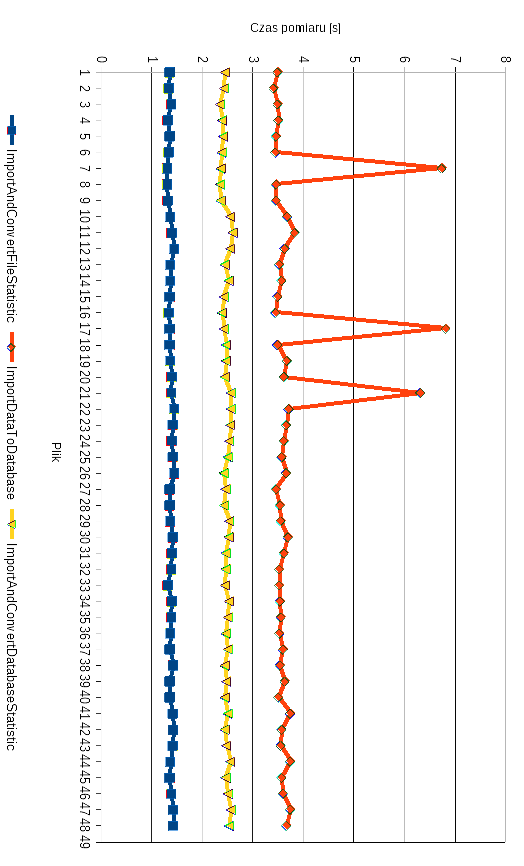
\includegraphics[width=\linewidth]{resources/statystyka_pomiaru.png}
    \caption{Przedstawienie wyników pomiaru czasu obsługi danych}
    \label{fig:importdata}
\end{figure}
\subsection{Porównanie algorytmów}
\label{ssec:compalgorithms}
Obserwując wyniki algorytmów zaprezentowane w sekcji \ref{ssec:queryparameters} można stwierdzić, że wyniki końcowe zależą dużo od wartości określonych w parametrach wewnętrznych. Niepoprawna wartość prędkości granicznej dla algorytmu I-VT, czy też wartości dyspersji i rozmiaru okna czasowego dla algorytmu I-DT może powodować zbyt duże nagromadzenie, lub wręcz przeciwnie zbyt małą ilość danych. Dlatego niezbędne jest znalezienie w trakcie weryfikacji danych, jeżeli istnieje taka możliwość odpowiedniej wartości tych parametrów.\par
Jak już zostało napisane w sekcji \ref{sssec:ivtresults}, w trakcie testów odkryto, iż prawidłowy parametr prędkości mieści się w bliskim sąsiedztwie wartości $v = 0.0005$. Możemy zaobserwować duże różnice wewnątrz wynikach końcowych, dlatego należy ten parametr dostosowywać w zależności od wykonanego pomiaru, najlepiej indywidualnie dla każdego elementu. Przykładowe wyniki tego algorytmu odpowiednio dla wartości parametru \emph{v} wynoszących \emph{0.0001, 0.005} oraz \emph{0.001} i \emph{0.01} dla pliku \emph{1\_03\_1310301904.cal} zaprezentowano w odpowiedniej kolejności na rysunkach \ref{fig:ivt1}, \ref{fig:ivt2}, \ref{fig:ivt3}, \ref{fig:ivt4}. Na rysunkach \ref{fig:ivt1} oraz \ref{fig:ivt3} możemy zaobserwować ruch sakadyczny występujący pomiędzy punktami, nie tylko prawidłowe fiksacje. Wynik otrzymany na rysunku \ref{fig:ivt4} posiada za małą liczbę otrzymanych elementów, dla takiej próbki danych. Wykrywa on tylko punkty bardzo długiego skupienia oka. Rysunek \ref{fig:ivt2} przedstawia precyzyjnie fiksacje, jednak ze względu na rzeczywiste drgania oka, wykrywa też więcej punktów niż te pokazane na rysunku \ref{fig:ivt4}.\par
Nie jest zaskakującym wynikiem czas trwania algorytmu, wraz z wykorzystaniem pamięciowym, gdyż jedno porównanie do następnego elementu w tablicy oraz dalsza praca nad grupami fiksacji, w wypadku poprawnie skonstruowanego kodu nie powinno stanowić dużej złożoności czasowej oraz pamięciowej. W porównaniu do algorytmów I-DT oraz ML wykonanie oraz złożoność pamięciowa tego algorytmu są najmniejsze, jednak wyniki przy niedokładnie dobranym parametrze $v$ są najmniej dokładne, gdyż potrafią fałszywie uwzględnić ruch sakadyczny jako fiksację.
\begin{figure}[H]
    \centering
    \captionsetup{justification=centering,margin=2cm}
    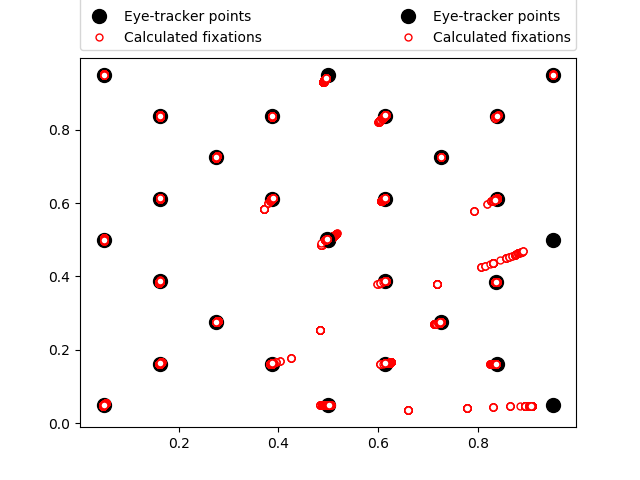
\includegraphics[width=0.8\linewidth]{resources/ivtresults/file1.png}
    \caption{Wynik algorytmu I-VT dla v = 0.0001}
    \label{fig:ivt1}
\end{figure}
\begin{figure}[H]
    \centering
    \captionsetup{justification=centering,margin=2cm}
    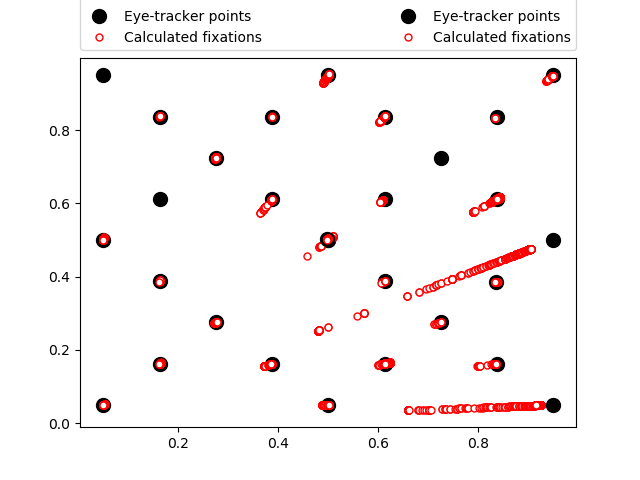
\includegraphics[width=0.8\linewidth]{resources/ivtresults/file2.png}
    \caption{Wynik algorytmu I-VT dla v = 0.0005}
    \label{fig:ivt2}
\end{figure}
\begin{figure}[H]
    \centering
    \captionsetup{justification=centering,margin=2cm}
    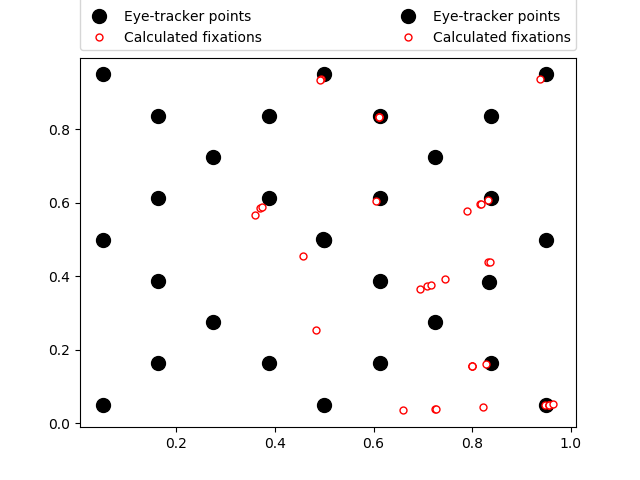
\includegraphics[width=0.8\linewidth]{resources/ivtresults/file3.png}
    \caption{Wynik algorytmu I-VT dla v = 0.001}
    \label{fig:ivt3}
\end{figure}
\begin{figure}[H]
    \centering
    \captionsetup{justification=centering,margin=2cm}
    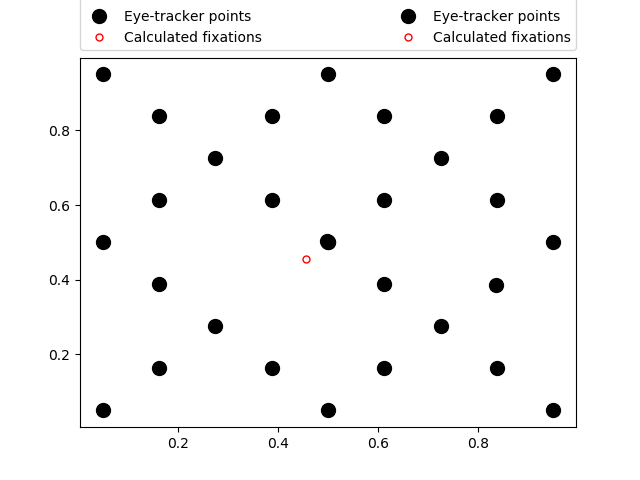
\includegraphics[width=0.8\linewidth]{resources/ivtresults/file4.png}
    \caption{Wynik algorytmu I-VT dla v = 0.01}
    \label{fig:ivt4}
\end{figure}
Analizując algorytm I-DT możemy wywnioskować, iż jest on najwolniejszy ze wszystkich algorytmów. Porównując wyniki tego algorytmu z algorytmami ML i I-VT, możemy również stwierdzić, iż jest on dość dokładny. Zaskakującym rezultatem jest podobieństwo w wykorzystaniu pamięci przez ten algorytm w porównaniu do algorytmu I-VT, ponieważ spodziewano się większego zużycia przez algorytm I-DT. Jak przedstawiono w wynikowych tabelach dotyczących algorytmu I-DT, większy wpływ na działanie algorytmu I-DT ma wartość parametru dyspersji. Czas okna służy tylko do stwierdzenia na jak długim wycinku danych ma być przeprowadzona analiza dyspersji. Przykładowy wynik algorytmu I-DT zaprezentowano na rysunku \ref{fig:idtresult}\par
\begin{figure}[H]
    \centering
    \captionsetup{justification=centering,margin=2cm}
    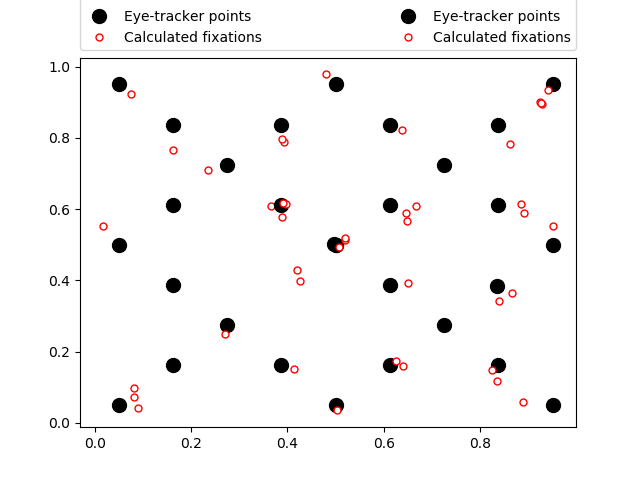
\includegraphics[width=0.8\linewidth]{resources/idt/idt-disp.png}
    \caption{Wynik algorytmu I-DT dla D = 0.05 i T = 200 ms)}
    \label{fig:idtresult}
\end{figure}
Algorytm uczenia maszynowego wymaga prawidłowego stworzenia modelu, by mógł on poprawnie funkcjonować. Porównując wyniki otrzymane za jego pomocą do tych otrzymanych za pomocą klasycznych algorytmów można stwierdzić, iż działa on dłużej od I-VT, ale zdecydowanie krócej od algorytmu I-DT, ale wykorzystuje on najwięcej pamięci operacyjnej do przygotowania obliczeń. Niebezpieczeństwem przy źle utworzonym modelu jest możliwość nieotrzymania danych wyjściowych, co zaprezentowano w tabelach umieszczonych w sekcji \ref{sssec:mlivt}. Patrząc na otrzymaną precyzję końcową da się określić, iż wybrane parametry modelu (prędkość międzypunktowa oraz odległość) są dobrze dobrane. Na rysunku XXX zaprezentowany został wynik końcowy dla pliku \emph{1\_03\_1310301904.cal} przy określeniu następujących parametrów: $v = 0.0005$ oraz proporcjach podziału modelu 35\%-65\%.
\begin{figure}[H]
    \centering
    \captionsetup{justification=centering,margin=2cm}
    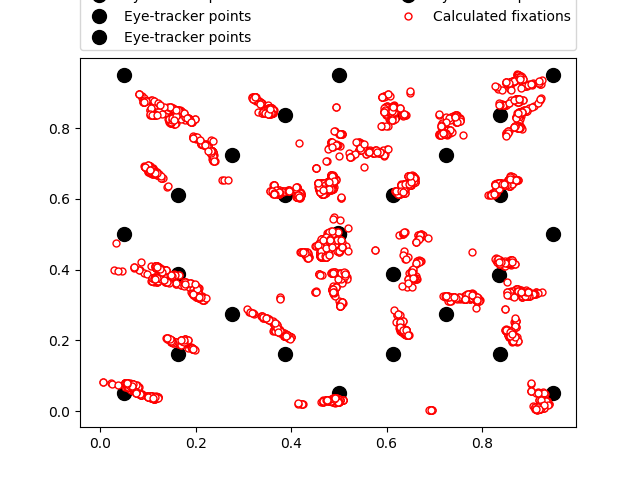
\includegraphics[width=0.8\linewidth]{resources/ml-result.png}
    \caption{Wynik algorytmu ML dla v = 0.0005 oraz P=(35\%-65\%)}
    \label{fig:mlresult}
\end{figure}
Pomimo podobnej liczby wykrytych punktów do algorytmu I-VT możemy zaobserwować większe nagromadzenie punktów w obliczonych fiksacjach przy właściwych punktach w stosunku do tych przedstawionych na rysunkach \ref{fig:ivt1}, \ref{fig:ivt2}, \ref{fig:ivt3}, \ref{fig:ivt4}. Przykład niepoprawnych wyników spowodowanych błędnym modelem zaprezentowano na rysunku \ref{fig:incorrectml}.
\begin{figure}[H]
    \centering
    \captionsetup{justification=centering,margin=2cm}
    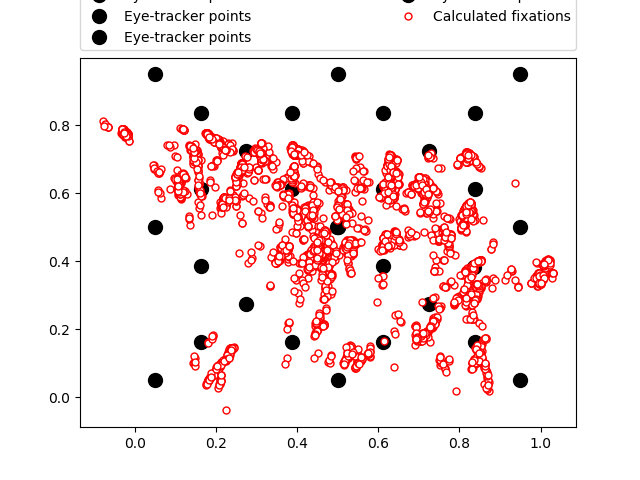
\includegraphics[width=0.8\linewidth]{resources/ml-incorrect.png}
    \caption{Wynik algorytmu ML dla v = 0.0005 oraz P=(50\%-50\%)}
    \label{fig:incorrectml}
\end{figure}
Na tym rysunku można zaobserwować punkty skupienia będące umieszczone zarówno w okolicach punktów, jak i w trakcie ruchu sakadowego.\par
Powyższe wyniki pozwalają nam określić, iż algorytm ML posiada najlepszy stosunek prędkości wykonywanych operacji do dokładności, i gdyby przeznaczyć ten projekt do dalszych celów badawczych, zalecane jest korzystanie z tego rozwiązania. Algorytm I-DT mimo, iż jest dokładny, wymaga dość dużego nakładu czasowego, gdyż wykonuje się prawie 100 razy więcej niż algorytmy I-VT i ML. Zaleca się z niego korzystać w przypadku mniejszej ilości danych. Natomiast algorytm I-VT jest dość niedokładny, co może powodować błędy w dalszej analizie punktów fiksacji. W celu poprawnego działania, proponuje się zastosowanie dla każdego z plików osobnej wartości prędkości, celem osiągnięcia lepszych rezultatów.